% Options for packages loaded elsewhere
\PassOptionsToPackage{unicode}{hyperref}
\PassOptionsToPackage{hyphens}{url}
\PassOptionsToPackage{dvipsnames,svgnames,x11names}{xcolor}
\documentclass[
  spanish,
  10pt,
  a4paper,
]{article}
\usepackage{xcolor}
\usepackage[top=22mm,bottom=22mm,left=22mm,right=22mm]{geometry}
\usepackage{amsmath,amssymb}
\setcounter{secnumdepth}{-\maxdimen} % remove section numbering
\usepackage{iftex}
\ifPDFTeX
  \usepackage[T1]{fontenc}
  \usepackage[utf8]{inputenc}
  \usepackage{textcomp} % provide euro and other symbols
\else % if luatex or xetex
  \usepackage{unicode-math} % this also loads fontspec
  \defaultfontfeatures{Scale=MatchLowercase}
  \defaultfontfeatures[\rmfamily]{Ligatures=TeX,Scale=1}
\fi
\usepackage{lmodern}
\ifPDFTeX\else
  % xetex/luatex font selection
\fi
% Use upquote if available, for straight quotes in verbatim environments
\IfFileExists{upquote.sty}{\usepackage{upquote}}{}
\IfFileExists{microtype.sty}{% use microtype if available
  \usepackage[]{microtype}
  \UseMicrotypeSet[protrusion]{basicmath} % disable protrusion for tt fonts
}{}
\usepackage{setspace}
\makeatletter
\@ifundefined{KOMAClassName}{% if non-KOMA class
  \IfFileExists{parskip.sty}{%
    \usepackage{parskip}
  }{% else
    \setlength{\parindent}{0pt}
    \setlength{\parskip}{6pt plus 2pt minus 1pt}}
}{% if KOMA class
  \KOMAoptions{parskip=half}}
\makeatother
\usepackage{longtable,booktabs,array}
\newcounter{none} % for unnumbered tables
\usepackage{calc} % for calculating minipage widths
% Correct order of tables after \paragraph or \subparagraph
\usepackage{etoolbox}
\makeatletter
\patchcmd\longtable{\par}{\if@noskipsec\mbox{}\fi\par}{}{}
\makeatother
% Allow footnotes in longtable head/foot
\IfFileExists{footnotehyper.sty}{\usepackage{footnotehyper}}{\usepackage{footnote}}
\makesavenoteenv{longtable}
\usepackage{graphicx}
\makeatletter
\newsavebox\pandoc@box
\newcommand*\pandocbounded[1]{% scales image to fit in text height/width
  \sbox\pandoc@box{#1}%
  \Gscale@div\@tempa{\textheight}{\dimexpr\ht\pandoc@box+\dp\pandoc@box\relax}%
  \Gscale@div\@tempb{\linewidth}{\wd\pandoc@box}%
  \ifdim\@tempb\p@<\@tempa\p@\let\@tempa\@tempb\fi% select the smaller of both
  \ifdim\@tempa\p@<\p@\scalebox{\@tempa}{\usebox\pandoc@box}%
  \else\usebox{\pandoc@box}%
  \fi%
}
% Set default figure placement to htbp
\def\fps@figure{htbp}
\makeatother
\ifLuaTeX
\usepackage[bidi=basic,shorthands=off]{babel}
\else
\usepackage[bidi=default,shorthands=off]{babel}
\fi
\ifLuaTeX
  \usepackage{selnolig} % disable illegal ligatures
\fi
\setlength{\emergencystretch}{3em} % prevent overfull lines
\providecommand{\tightlist}{%
  \setlength{\itemsep}{0pt}\setlength{\parskip}{0pt}}

\usepackage{amsmath,amssymb,mathtools}
\usepackage{microtype}
\usepackage{fancyhdr}
\usepackage{needspace}
\usepackage{etoolbox}
\usepackage{float}
\usepackage{caption}
\captionsetup{font=small,labelformat=empty,skip=7pt}
\floatplacement{figure}{H}
\definecolor{DocBlue}{HTML}{173F57}
\definecolor{DocGray}{HTML}{52616C}
\pagestyle{fancy}
\fancyhf{}
\fancyhead[L]{\small\sffamily\color{DocGray} pySNSPD | Desarrollo del modelo}
\fancyhead[R]{\small\sffamily\color{DocGray} Modelo 0.4 | E-r02}
\fancyfoot[L]{\small\sffamily\color{DocGray} 9 de septiembre de 2026}
\fancyfoot[R]{\small\sffamily\thepage}
\setlength{\headheight}{15pt}
\setlength{\emergencystretch}{2em}
\setlength{\parskip}{5pt plus 1pt}
\setlength{\parindent}{0pt}
\widowpenalty=10000
\clubpenalty=10000
\displaywidowpenalty=10000
\predisplaypenalty=10000
\renewcommand{\arraystretch}{1.16}
\AtBeginEnvironment{longtable}{\small}
\pretocmd{\section}{\Needspace{6\baselineskip}}{}{}
\pretocmd{\subsection}{\Needspace{5\baselineskip}}{}{}
\AtBeginDocument{\hypersetup{colorlinks=true,linkcolor=DocBlue,urlcolor=DocBlue}}
\allowdisplaybreaks[1]
\usepackage{bookmark}
\IfFileExists{xurl.sty}{\usepackage{xurl}}{} % add URL line breaks if available
\urlstyle{same}
\hypersetup{
  pdftitle={E. Cuaderno de aprendizaje del modelo},
  pdflang={es},
  colorlinks=true,
  linkcolor={Maroon},
  filecolor={Maroon},
  citecolor={Blue},
  urlcolor={Blue},
  pdfcreator={LaTeX via pandoc}}

\title{E. Cuaderno de aprendizaje del modelo}
\usepackage{etoolbox}
\makeatletter
\providecommand{\subtitle}[1]{% add subtitle to \maketitle
  \apptocmd{\@title}{\par {\large #1 \par}}{}{}
}
\makeatother
\subtitle{Clases autónomas · Edición del modelo 0.4}
\author{}
\date{9 de septiembre de 2026 · Cuaderno E-r02}

\begin{document}
\maketitle

{
\setcounter{tocdepth}{1}
\tableofcontents
}
\setstretch{1.07}
\newpage

\setlength{\parskip}{4pt plus 1pt}

\section{E.0. Ruta y registro de
aprendizaje}\label{e.0.-ruta-y-registro-de-aprendizaje}

Cada clase parte de un sistema concreto, presenta sus variables y
desarrolla un ejemplo antes de proponer actividades. Puede leerse de
manera aislada: los conceptos necesarios se recuperan en el propio
texto. La tabla ofrece material previo recomendado, sin darlo por
dominado ni exigir una lectura lineal. Las relaciones entre clases se
expresan al volver a usar las ideas; los códigos se reservan para
orientarse y registrar respuestas.

{\def\LTcaptype{none} % do not increment counter
\begin{longtable}[]{@{}
  >{\raggedright\arraybackslash}p{(\linewidth - 6\tabcolsep) * \real{0.2500}}
  >{\raggedright\arraybackslash}p{(\linewidth - 6\tabcolsep) * \real{0.2500}}
  >{\raggedright\arraybackslash}p{(\linewidth - 6\tabcolsep) * \real{0.2500}}
  >{\raggedright\arraybackslash}p{(\linewidth - 6\tabcolsep) * \real{0.2500}}@{}}
\toprule\noalign{}
\begin{minipage}[b]{\linewidth}\raggedright
ID estable
\end{minipage} & \begin{minipage}[b]{\linewidth}\raggedright
Clase
\end{minipage} & \begin{minipage}[b]{\linewidth}\raggedright
Estado
\end{minipage} & \begin{minipage}[b]{\linewidth}\raggedright
Material previo recomendado
\end{minipage} \\
\midrule\noalign{}
\endhead
\bottomrule\noalign{}
\endlastfoot
E01 & Sistemas, campos, estados y excitaciones & ABIERTO & Posición y
velocidad; vectores; corriente y tensión \\
E04 & Electrones y huecos: materiales y fronteras & ABIERTO & E01; carga
eléctrica; corriente convencional; energía potencial \\
E06 & Ocupaciones y operadores & ABIERTO & E01, E04; matrices;
derivadas; mecánica de una masa y un resorte \\
E07 & Una columna de Nambu & ABIERTO & E04, E06; números complejos;
valores propios \\
E03 & Variar una energía funcional & ABIERTO & E01; derivadas; regla del
producto y de la cadena; integración por partes \\
E05 & Modos, distribuciones y DOS & ABIERTO & E01; oscilador armónico;
integrales; valores propios; probabilidad básica \\
E09 & DFT: densidad y estructura electrónica & ABIERTO & E01, E03, E04,
E05; normalización; potencial y energía; orbitales \\
E10 & DFPT: respuesta e interacción electrón--fonón & ABIERTO & E03,
E05, E09; E07 para el factor superconductor; Taylor; unidades y
conservación de energía \\
\end{longtable}
}

Los números E01, E03, etc. son identificadores permanentes; E.1, E.2,
etc. sólo indican el orden de lectura. E02 está descartada y fue
sustituida por E06/E07. E08 se retira y se sustituye por las nuevas E09
(DFT) y E10 (DFPT). No se asignan actividades ni se recomienda estudiar
las clases retiradas. Su retiro es una decisión editorial, no una
evaluación del aprendizaje.

No hay respuestas entregadas ni calificaciones asignadas. Cada clase
propone tres actividades, por 4, 3 y 3 puntos; se cierra con al menos 8
puntos y su condición esencial satisfecha. Los ejemplos resueltos son
distintos de esas actividades. Las observaciones de lectura sirven para
revisar la enseñanza y no se califican como respuestas incorrectas. Las
respuestas futuras y su evidencia se conservan aunque se revise una
clase; si cambia una consigna, se conserva también su versión anterior.

\textbf{Revisión de esta entrega:} E01, E03, E04, E05, E06 y E07 pasan
de r1 a r2; E09 y E10 comienzan en r1. El cuaderno ensamblado es E-r02 y
sigue perteneciendo a la edición del modelo 0.4. Una corrección
posterior incrementará sólo la revisión de las clases afectadas y la del
ensamblado; no cambiará automáticamente A--D ni la versión del modelo.
Las ecuaciones antiguas conservan sus etiquetas; las nuevas usan el
código de su clase para que añadir contenido no renumere las demás. El
historial y la regla completa se guardan junto al documento editable.

\clearpage

\section{E.1. Sistemas, campos, estados y excitaciones ---
E01}\label{e.1.-sistemas-campos-estados-y-excitaciones-e01}

\textbf{Revisión: r2. Estado: ABIERTO. Meta:} distinguir qué se está
describiendo antes de interpretar masa, carga o espín.

\subsection{E.1.1. Introducción}\label{e.1.1.-introducciuxf3n}

Un \textbf{sistema} es la parte del mundo que decidimos describir: una
masa sujeta a un resorte, una cavidad electromagnética o un tramo de
conductor conectado a una fuente. Elegimos sus límites, las
interacciones relevantes y las variables que responden a nuestra
pregunta. En mecánica, una coordenada \(q(t)\) puede indicar la
\textbf{posición} de una masa; su desplazamiento respecto de una
posición de referencia \(q_0\) es \(u(t)=q(t)-q_0\). Otras coordenadas
posibles son un ángulo o la elongación de un resorte. Coordenada y
desplazamiento sólo coinciden si se elige así la referencia.

Un \textbf{campo} asigna un valor a cada punto de un dominio. Por
ejemplo, \(T(\mathbf r,t)\) asigna una temperatura a cada posición
\(\mathbf r=(x,y,z)\) y a cada instante \(t\). El valor puede ser un
número, como \(T\), o varias componentes: el desplazamiento elástico
\(\mathbf u(\mathbf r,t)=(u_x,u_y,u_z)\) asigna un vector a cada punto.
Las componentes son los valores que toma el campo; \(\mathbf r\) y \(t\)
son las coordenadas donde se lo evalúa. El campo eléctrico
\(\mathbf E(\mathbf r,t)\) también es vectorial y no representa por eso
la trayectoria de una partícula.

Una \textbf{configuración} es una elección de todos esos valores a un
instante: el perfil completo de temperatura, por ejemplo. En una
descripción clásica, el \textbf{estado} reúne los datos que el modelo
necesita para continuar la evolución. Puede ser la configuración de un
campo o de varios campos definidos en un mismo dominio, si éstos bastan.
Para una cuerda vibrante se necesitan tanto \(u(x,t_0)\) como su
velocidad \(\partial_tu(x,t_0)\); dos cuerdas con el mismo perfil y
velocidades opuestas evolucionarán de manera distinta. Tampoco es
obligatorio que todas las variables compartan dominio: un dispositivo
puede combinar campos en un conductor con corrientes y tensiones de
circuito que sólo dependen del tiempo. En una descripción cuántica, el
estado incluye además la información probabilística y las correlaciones:
no se reduce en general a asignar números clásicos a cada punto.

Un \textbf{modo} es una forma independiente de variación admitida por el
modelo y sus condiciones de borde. En una cuerda fija en \(x=0,L\), una
forma posible es \(\phi_1(x)=\sin(\pi x/L)\); su amplitud temporal
\(a_1(t)\) determina cuánto participa en \(u(x,t)=a_1(t)\phi_1(x)\). Una
\textbf{excitación} es una desviación respecto de un estado de
referencia. Clásicamente puede consistir en aumentar esa amplitud; en el
oscilador cuántico consiste en cambiar la ocupación de niveles separados
por la energía del modo. Es útil separar, por tanto, sistema, variables,
estado, modos disponibles y excitaciones efectivamente presentes.

\begin{figure}
\centering
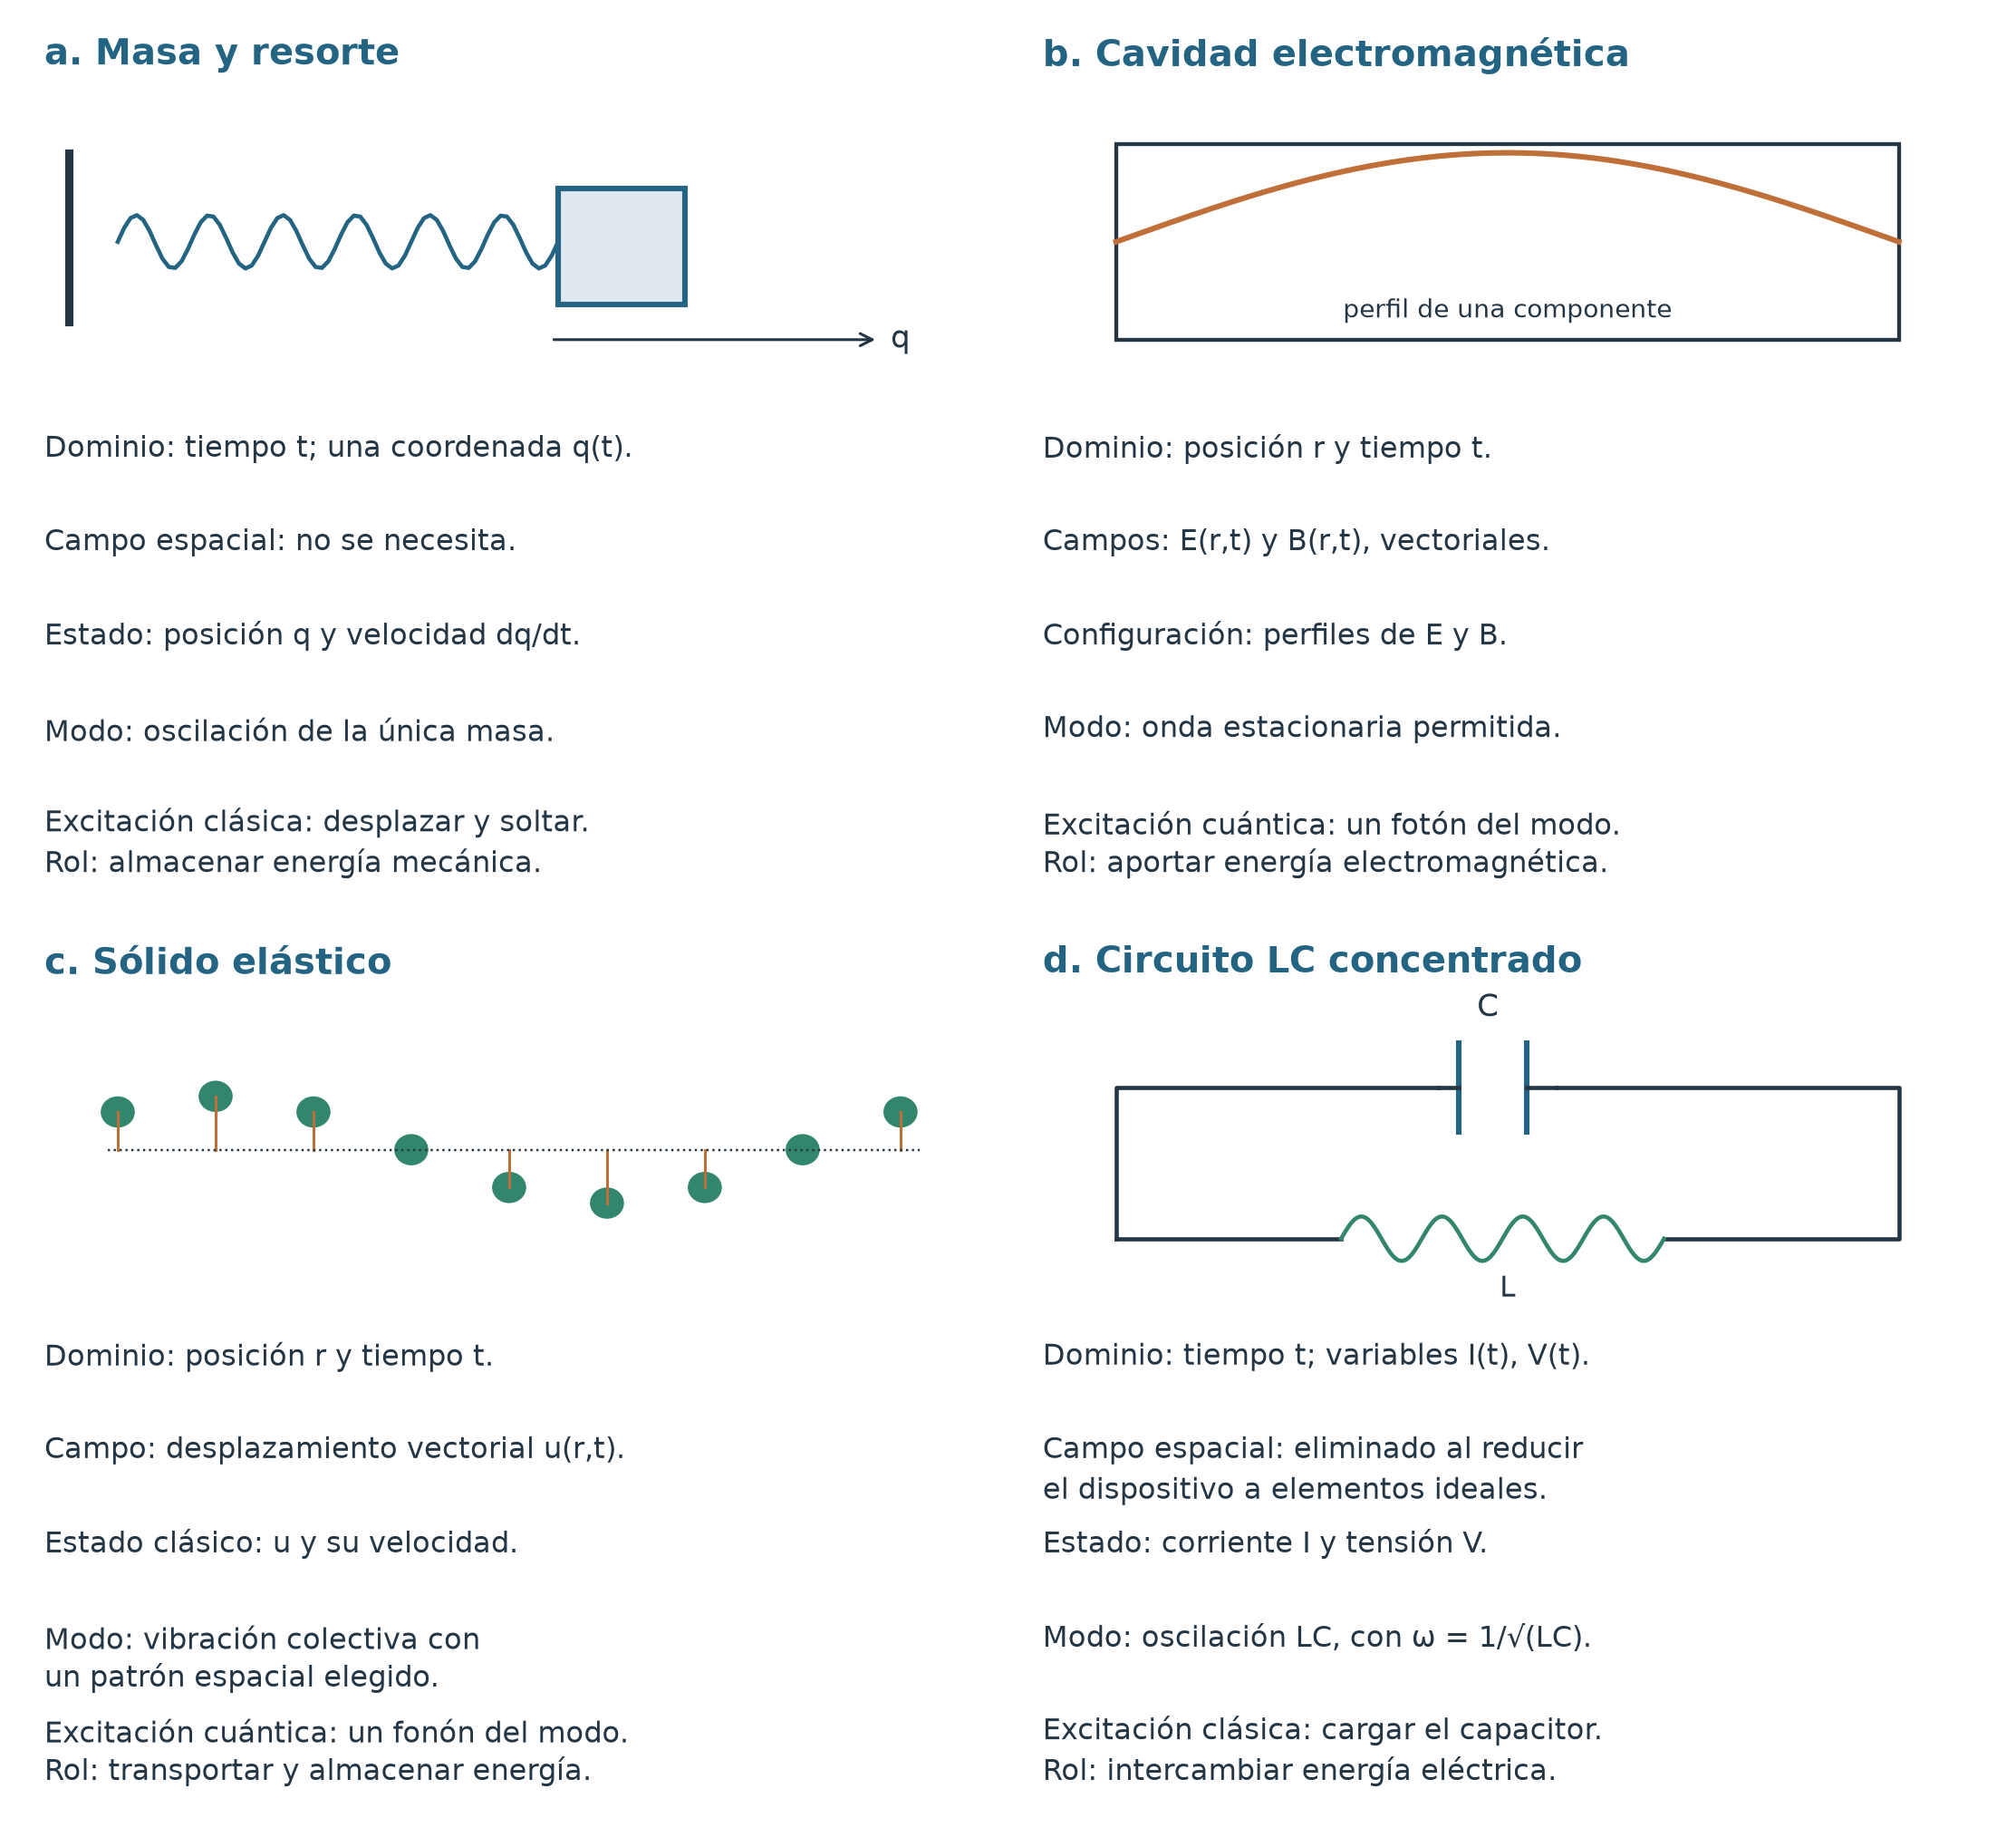
\includegraphics[width=1\linewidth,height=\textheight,keepaspectratio,alt={Figura E01.1. Un mismo lenguaje con objetos diferentes. En cada panel se identifican el sistema, el dominio, las variables, un modo y una excitación. El resorte puntual y el circuito concentrado no necesitan un campo espacial; la cavidad y el sólido sí admiten esa descripción. Son ejemplos ideales de elaboración propia.}]{../figuras/E01_sistemas_campos.png}
\caption{Figura E01.1. Un mismo lenguaje con objetos diferentes. En cada
panel se identifican el sistema, el dominio, las variables, un modo y
una excitación. El resorte puntual y el circuito concentrado no
necesitan un campo espacial; la cavidad y el sólido sí admiten esa
descripción. Son ejemplos ideales de elaboración propia.}
\end{figure}

En el sólido, \(\mathbf u(\mathbf r,t)\) describe desplazamientos de los
átomos y un fonón es un cuanto de un modo vibratorio. Para describir un
condensado superconductor se usa otro campo, \(\Delta(\mathbf r,t)\),
cuyo valor complejo tiene amplitud y fase. Una variación de su amplitud
o de su fase es colectiva; una cuasipartícula electrónica es otro tipo
de excitación. Qué variables se conservan depende de si queremos
estudiar vibración, emparejamiento o respuesta eléctrica.

El Modelo Estándar organiza campos elementales y sus interacciones
electromagnética, débil y fuerte. Los quarks y leptones son fermiones.
Un \textbf{modo fermiónico completamente especificado}, incluido su
espín, puede estar desocupado (\(n=0\): ningún fermión en ese modo) u
ocupado (\(n=1\): un fermión en ese modo). Un orbital que admite dos
orientaciones de espín contiene dos modos diferentes y puede alojar un
electrón en cada uno. En un modo bosónico, como un modo de luz, las
ocupaciones posibles son \(n=0,1,2,\ldots\). El modo es la posibilidad
disponible; su ocupación es parte de la descripción del estado. La tabla
muestra ejemplos, no el inventario completo.

\Needspace{10\baselineskip}

{\def\LTcaptype{none} % do not increment counter
\begin{longtable}[]{@{}llll@{}}
\toprule\noalign{}
Familia & Ejemplos & Carga eléctrica, en unidades de \(e>0\) & Espín \\
\midrule\noalign{}
\endhead
\bottomrule\noalign{}
\endlastfoot
Quarks & up, down & \(+2/3\), \(-1/3\) & \(1/2\) \\
Leptones & electrón, neutrino & \(-1\), \(0\) & \(1/2\) \\
Bosones asociados a interacciones & fotón, \(W^+\) & \(0\), \(+1\) &
\(1\) \\
Bosón de Higgs & Higgs & \(0\) & \(0\) \\
\end{longtable}
}

La especie identifica propiedades compartidas: todos los electrones
tienen la misma masa y carga. El espín es una propiedad de momento
angular intrínseco. Masa, carga y espín no especifican por sí solos el
estado de movimiento, la ocupación o las correlaciones. El Modelo
Estándar tampoco incluye una teoría cuántica completa de la gravedad. Un
protón es compuesto; un fonón es una excitación colectiva de un sólido,
no otra partícula elemental de esa tabla.

\subsection{E.1.2. Ejemplo resuelto}\label{e.1.2.-ejemplo-resuelto}

\textbf{Problema:} un protón contiene quarks de valencia up, up, down.
¿Qué se puede obtener sumando los datos de carga?

La suma es \(2/3+2/3-1/3=1\): carga \(+e\). Si se añade un electrón de
carga \(-e\), el conjunto tiene carga neta cero. Eso no determina la
masa, la energía de enlace ni el estado cuántico. La carga es aditiva;
la energía de un sistema ligado incluye interacciones. En particular,
sumar tres números de espín \(1/2\) tampoco determina el espín del
protón: hay que conocer cómo se combinan los momentos angulares.

\subsection{E.1.3. Actividad}\label{e.1.3.-actividad}

\Needspace{4\baselineskip}

\textbf{E01.1, 4 puntos.} Un neutrón tiene quarks de valencia up, down,
down. Calcular su carga con la tabla e indicar una propiedad que no
queda determinada por esa suma.

\textbf{Respuesta E01.1:} \emph{Escribir aquí.}

\Needspace{4\baselineskip}

\textbf{E01.2, 3 puntos.} Clasificar electrón, protón, fonón y corriente
de una inductancia como especie elemental, objeto compuesto, excitación
colectiva o variable de circuito.

\textbf{Respuesta E01.2:} \emph{Escribir aquí.}

\Needspace{4\baselineskip}

\textbf{E01.3, 3 puntos.} Corregir: «si dos electrones tienen igual
masa, carga y espín, están necesariamente en el mismo estado cuántico».

\textbf{Respuesta E01.3:} \emph{Escribir aquí.}

\textbf{Condición esencial:} separar especie, estado cuántico y variable
efectiva.

\textbf{Fuentes:}
\href{https://home.cern/science/physics/standard-model/}{CERN, Modelo
Estándar} y
\href{https://ocw.mit.edu/courses/8-03sc-physics-iii-vibrations-and-waves-fall-2016/}{MIT
8.03, modos normales y ondas}. Los sistemas, el esquema y el ejercicio
se construyen aquí para distinguir las descripciones.

\Needspace{14\baselineskip}

\bigskip

\section{E.2. Electrones y huecos: elegir la referencia ---
E04}\label{e.2.-electrones-y-huecos-elegir-la-referencia-e04}

\textbf{Revisión: r2. Estado: ABIERTO. Meta:} reconocer qué conduce en
cuatro materiales y contabilizar carga y energía respecto de una
referencia.

\subsection{E.2.1. Introducción: del elemento de circuito a sus
portadores}\label{e.2.1.-introducciuxf3n-del-elemento-de-circuito-a-sus-portadores}

Un sistema puede ser el trozo de material entre dos terminales. El
circuito lo describe mediante tensión y corriente; su descripción
microscópica incluye una red de átomos y los electrones que la ocupan.
Un \textbf{modo electrónico} es una forma permitida de la onda del
electrón, con una energía y un espín especificados. En un cristal,
muchos modos forman familias cuyas energías recorren intervalos llamados
\textbf{bandas}. Una banda reúne modos disponibles: todavía hay que
indicar cuáles están ocupados. No es una franja del espacio ni una
trayectoria del electrón.

En un semiconductor intrínseco ideal, la \textbf{banda de valencia} está
llena a temperatura cero y la \textbf{banda de conducción} vacía. Sus
bordes, \(E_v\) y \(E_c\), están separados por una brecha de energías
sin modos electrónicos extendidos del cristal ideal: \(E_g=E_c-E_v\). A
temperatura finita o al absorber luz, un electrón puede pasar a
conducción y dejar un modo de valencia vacío. Esa ausencia respecto de
la banda llena se llama \textbf{hueco}. El electrón de conducción y el
hueco de valencia pueden contribuir al transporte.
\href{https://ocw.mit.edu/courses/3-091sc-introduction-to-solid-state-chemistry-fall-2010/pages/electronic-materials/14-semiconductors/}{MIT,
bandas y portadores}.

Consideremos cuatro situaciones. En la resistencia metálica hay modos
ocupados y vacíos próximos en energía; un campo eléctrico modifica
ligeramente su ocupación y produce deriva electrónica. La dispersión por
desorden y vibraciones limita la corriente; en régimen estacionario, la
potencia eléctrica \(IV\) termina como calor. En el semiconductor
\textbf{intrínseco}, sin dopaje intencional, la generación produce un
electrón y un hueco, de modo que sus concentraciones son iguales en
equilibrio. En el semiconductor \textbf{dopado tipo n}, donantes
ionizados aportan electrones móviles y quedan como cargas positivas
fijas. El tipo p se obtiene con aceptores: predominan los huecos y
quedan aceptores negativos fijos. El dopaje permite cambiar las
concentraciones sin generar siempre parejas electrón--hueco.
\href{https://ocw.mit.edu/courses/6-012-microelectronic-devices-and-circuits-spring-2009/6583f0018f5bb90464ea68b550f73c95_MIT6_012S09_lec02.pdf}{MIT,
generación y dopaje, pp.~5--13}.

En el superconductor convencional, el estado electrónico colectivo
incluye pares correlacionados que forman un \textbf{condensado}. Éste
puede sostener corriente continua sin caída resistiva mientras se
mantenga el régimen superconductor. Sus excitaciones adicionales se
llaman \textbf{cuasipartículas} (QP) y transportan energía; su contenido
electrónico y de hueco también interviene en la respuesta eléctrica. La
supercorriente no requiere una población de QP. La brecha \(\Delta\) es
aquí el umbral para una QP en el caso uniforme de brecha completa; crear
dos requiere al menos \(2\Delta\). No es la separación \(E_g\) entre
valencia y conducción.
\href{https://journals.aps.org/pr/abstract/10.1103/PhysRev.108.1175}{Bardeen,
Cooper y Schrieffer, teoría microscópica}.

Por tanto, \textbf{semiconductor} describe una estructura de bandas y
unos portadores controlables; \textbf{superconductor} describe un estado
colectivo con respuesta eléctrica y magnética propia. No son grados
sucesivos de conductividad. Un material semiconductor también puede
adquirir superconductividad en determinadas condiciones: ambas palabras
responden a preguntas diferentes.

\begin{figure}
\centering
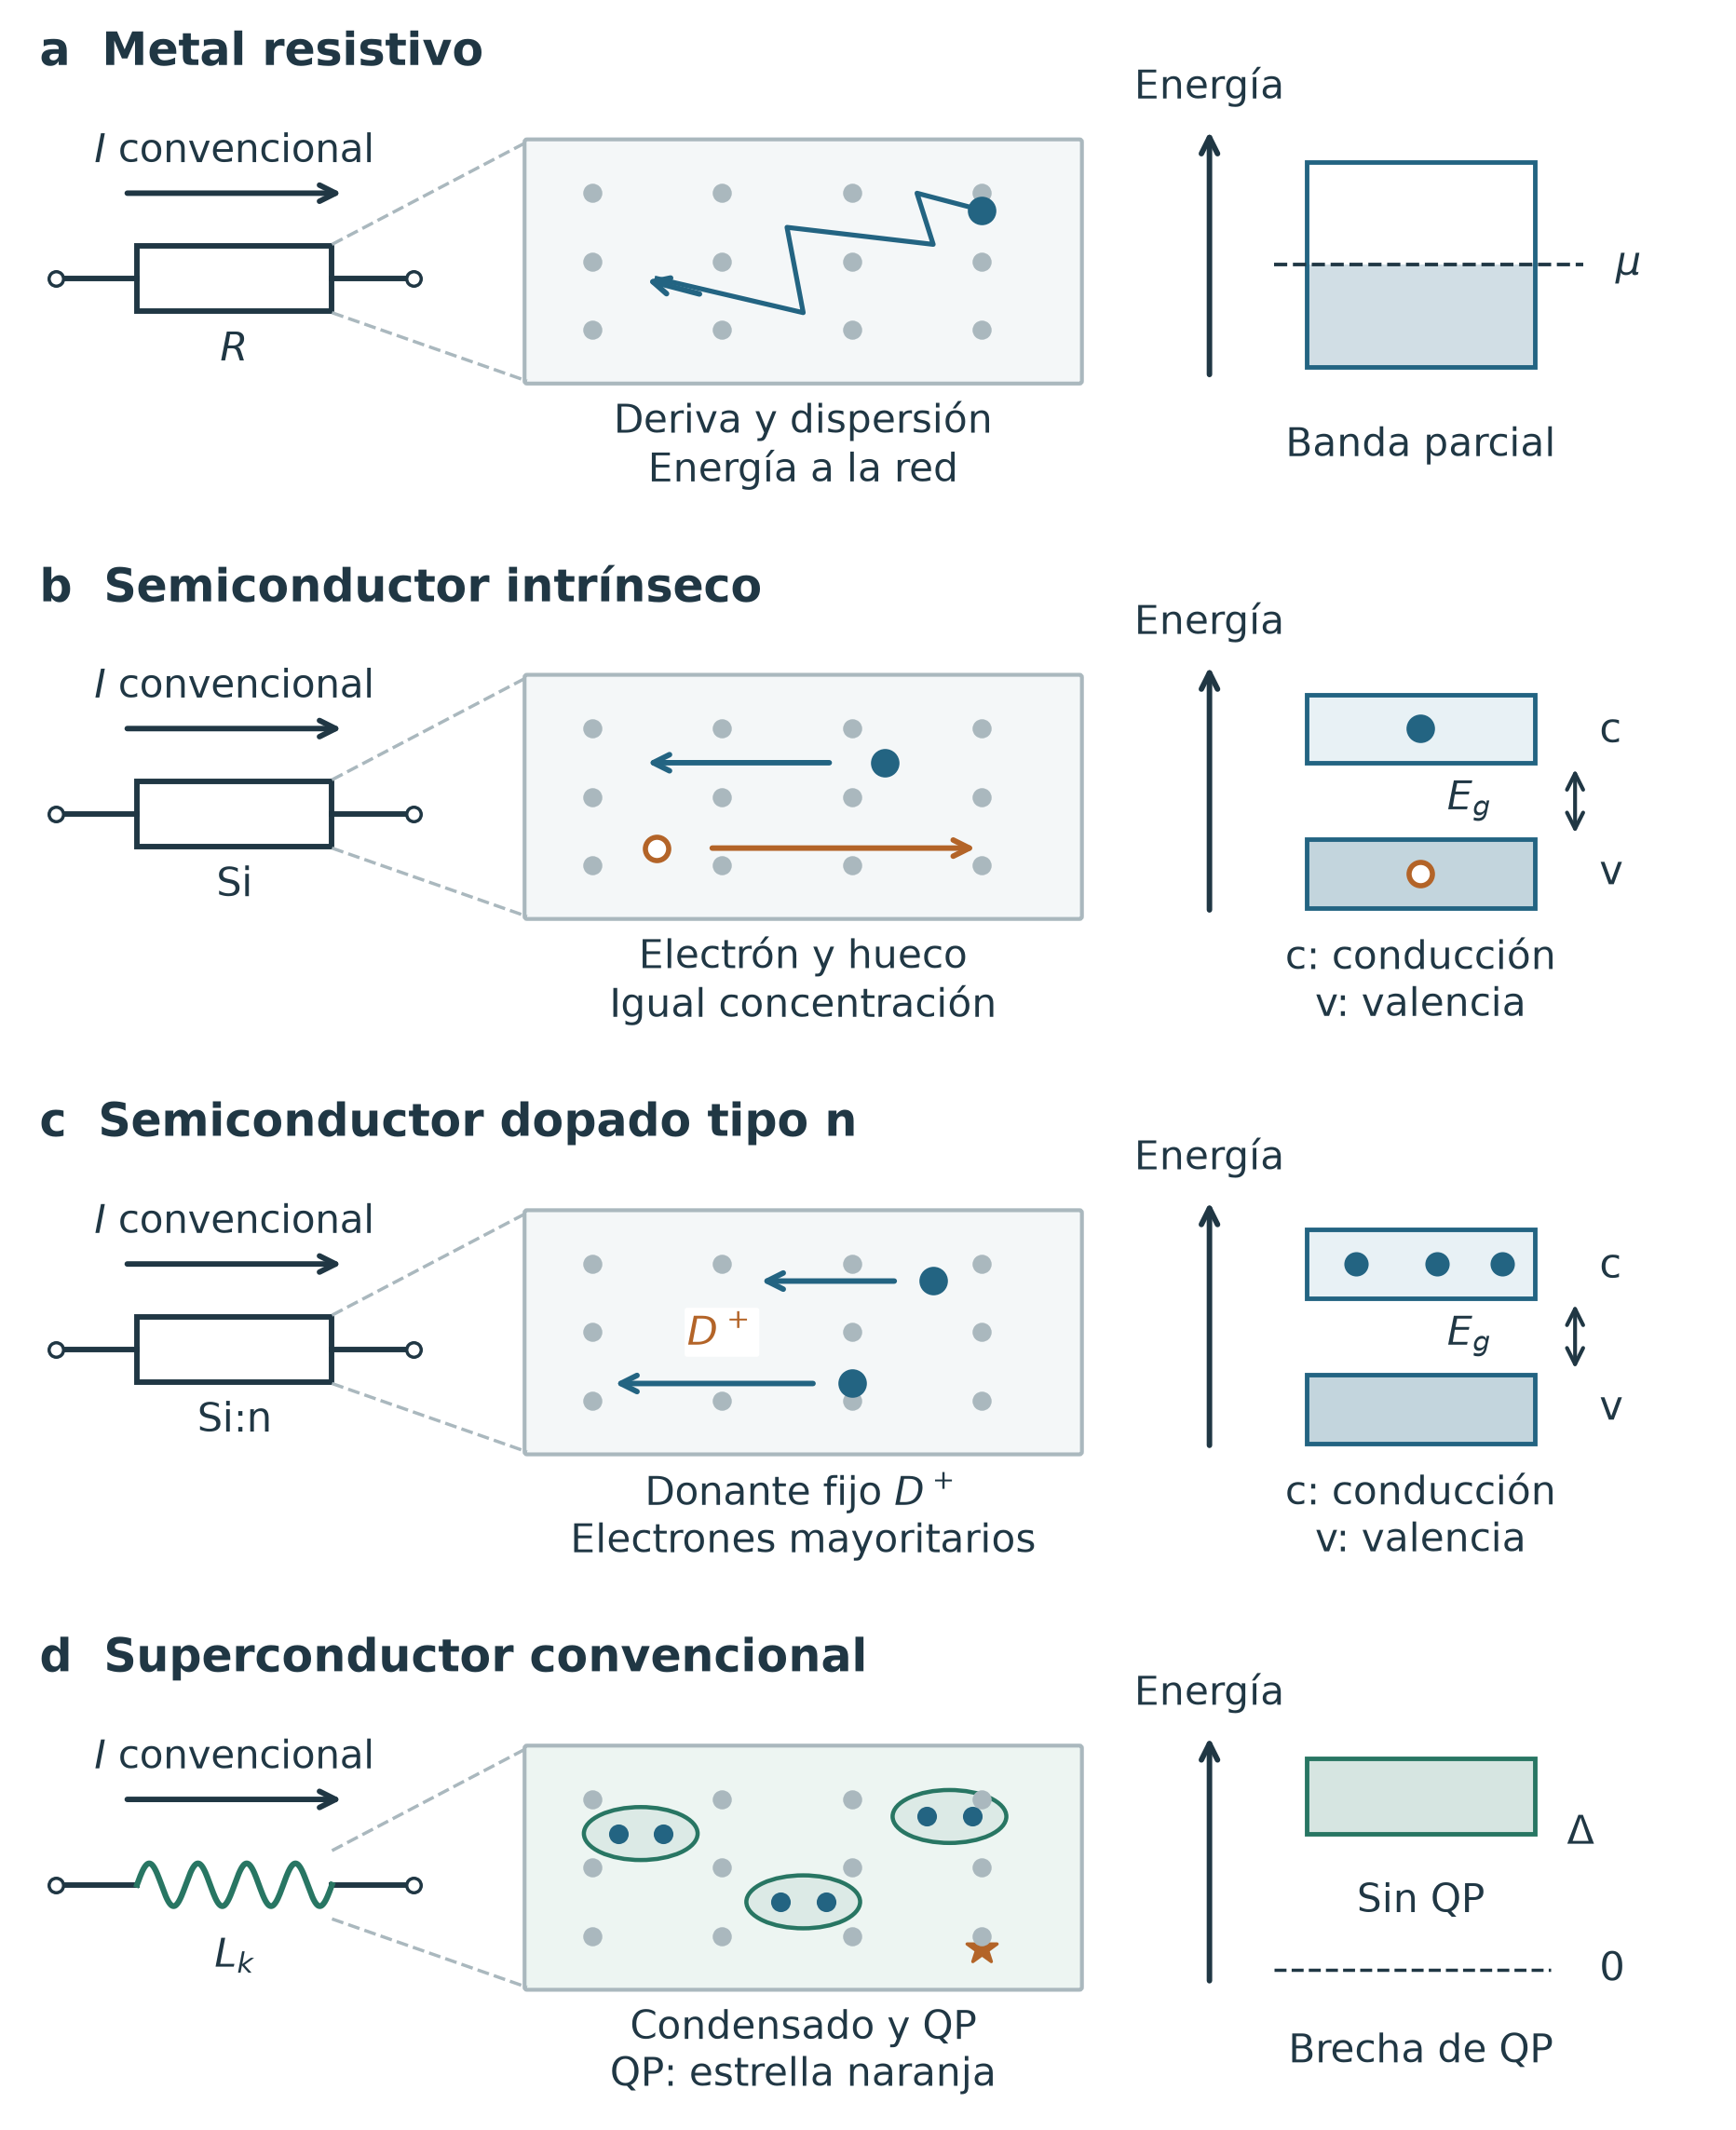
\includegraphics[width=1\linewidth,height=\textheight,keepaspectratio,alt={Figura E.2a. Elemento de circuito, ampliación microscópica y energías. Puntos grises: centros de la red; azules: electrones; blancos: huecos. Las parejas simbolizan correlaciones del condensado, no moléculas separadas. Sin escala atómica. \textbackslash mu es el potencial químico, una referencia energética. El último panel muestra energías positivas de cuasipartículas (QP); la bobina representa la inductancia cinética L\_k, debida a la respuesta inercial de los portadores.}]{../figuras/E04_circuitos_micro.png}
\caption{Figura E.2a. Elemento de circuito, ampliación microscópica y
energías. Puntos grises: centros de la red; azules: electrones; blancos:
huecos. Las parejas simbolizan correlaciones del condensado, no
moléculas separadas. Sin escala atómica. \(\mu\) es el potencial
químico, una referencia energética. El último panel muestra energías
positivas de cuasipartículas (QP); la bobina representa la inductancia
cinética \(L_k\), debida a la respuesta inercial de los portadores.}
\end{figure}

Para entender por qué sirve contar huecos, se puede empezar por una
banda de juguete con 12 modos, cada uno con espín ya especificado. Su
ocupación \(n_i\) vale 1 si el modo \(i\) contiene un electrón y 0 si
está vacío. Si sólo faltan los electrones de los modos 4 y 10,

\[
\begin{aligned}
(n_1,\ldots,n_{12})&=(1,1,1,0,1,1,1,1,1,0,1,1),\\
h_i&=1-n_i,\qquad H=\sum_{i=1}^{12}h_i=2,\\
N&=\sum_{i=1}^{12}n_i=12-H=10.
\end{aligned}
\tag{E04.a}
\]

Una lista de electrones necesita diez índices; la lista de huecos sólo
necesita \(\{4,10\}\) y la referencia «los doce modos llenos». Al
rellenar el modo 4 y vaciar el 5, basta cambiar \(\{4,10\}\) por
\(\{5,10\}\). Los índices identifican modos; no son necesariamente
posiciones vecinas. La reducción es exacta: con \(10^6\) modos y 3
huecos, se almacenan tres índices en vez de 999 997, una vez conocida la
referencia. Esto simplifica el registro de ocupaciones; no elimina la
necesidad de calcular sus energías o interacciones.

También se simplifica una suma física. En una banda completa, las
contribuciones de velocidades opuestas se cancelan. Como ejemplo de esa
cancelación, cuatro modos tienen velocidades \(v_i/v_0=(-3,-1,1,3)\),
donde \(v_0>0\) fija la unidad de velocidad. Si falta sólo el tercero,
la suma electrónica es \(-3-1+3=-1\). El aporte total de los electrones
a \(\sum q_i v_i\) es entonces \((-e)(-v_0)=+ev_0\). Esta suma es
proporcional a la corriente en una geometría fija. Contando sólo la
vacante se obtiene el mismo resultado: \((+e)(+v_0)=+ev_0\). La carga
positiva del hueco reproduce exactamente el aporte que falta respecto de
la banda llena; no introduce otra especie elemental.

\subsection{E.2.2. La referencia fija la carga y la
energía}\label{e.2.2.-la-referencia-fija-la-carga-y-la-energuxeda}

En una imagen local simplificada, si un electrón de la derecha ocupa una
vacante de la izquierda, el electrón se movió a la izquierda y la
vacante a la derecha. La corriente convencional apunta a la derecha:
tiene sentido opuesto al movimiento de la carga negativa y el mismo que
el de la vacante positiva. En un cristal, esa imagen ayuda a seguir el
signo, aunque un modo electrónico pueda abarcar muchos átomos.

Para calcular se definen \(\varepsilon\) como energía de un nivel
electrónico, \(\mu\) como potencial químico de referencia y \(\delta N\)
como cambio del número de electrones: \(+1\) al añadir y \(-1\) al
retirar. La carga relativa es \(\delta Q=-e\delta N\), con \(e>0\). En
el modelo de niveles independientes, manteniendo fija la referencia, la
energía de excitación es el cambio de \(U-\mu N\):

\[
\delta E_{\rm exc}=(\varepsilon-\mu)\delta N,
\qquad \delta Q=-e\delta N.
\tag{E.1}
\]

La energía se mide respecto de la configuración de referencia: niveles
ocupados por debajo de \(\mu\) y vacíos por encima. Retirar un electrón
de un nivel ocupado con \(\varepsilon<\mu\) multiplica dos signos
negativos y cuesta energía positiva. Un hueco en el sólido no es un
positrón. Esta contabilidad describe adiciones y retiradas de electrones
normales; una QP superconductora mezcla ambas operaciones y requiere su
propia energía de excitación.

\textbf{Ejemplo resuelto.} Añadir un electrón a \(\varepsilon-\mu=3\)
meV da \(\delta E_{\rm exc}=3\) meV y \(\delta Q=-e\). Retirar otro a
\(\varepsilon-\mu=-2\) meV da \((-2)(-1)=2\) meV y \(\delta Q=+e\). El
conjunto contiene 5 meV de excitaciones y carga neta cero. Neutralidad
no significa ausencia de energía.

\subsection{E.2.3. Dos fronteras: p--n y
normal--superconductor}\label{e.2.3.-dos-fronteras-pn-y-normalsuperconductor}

En una unión \textbf{p--n} se encuentran dos regiones del semiconductor
con distintos dopajes. La difusión inicial y la recombinación dejan una
región empobrecida en portadores móviles, con dopantes ionizados fijos.
Aparece un campo eléctrico dirigido de n hacia p.~En equilibrio, las
corrientes de deriva y difusión se compensan. Una tensión directa reduce
la barrera e inyecta electrones de n hacia p y huecos de p hacia n; la
recombinación posterior libera energía. La brecha local entre bandas
puede seguir siendo \(E_g\) mientras ambos bordes se curvan con la
posición.
\href{https://ocw.mit.edu/courses/6-012-microelectronic-devices-and-circuits-fall-2005/pages/lecture-notes/}{MIT,
electrostática y transporte de la unión p--n}.

\begin{figure}
\centering
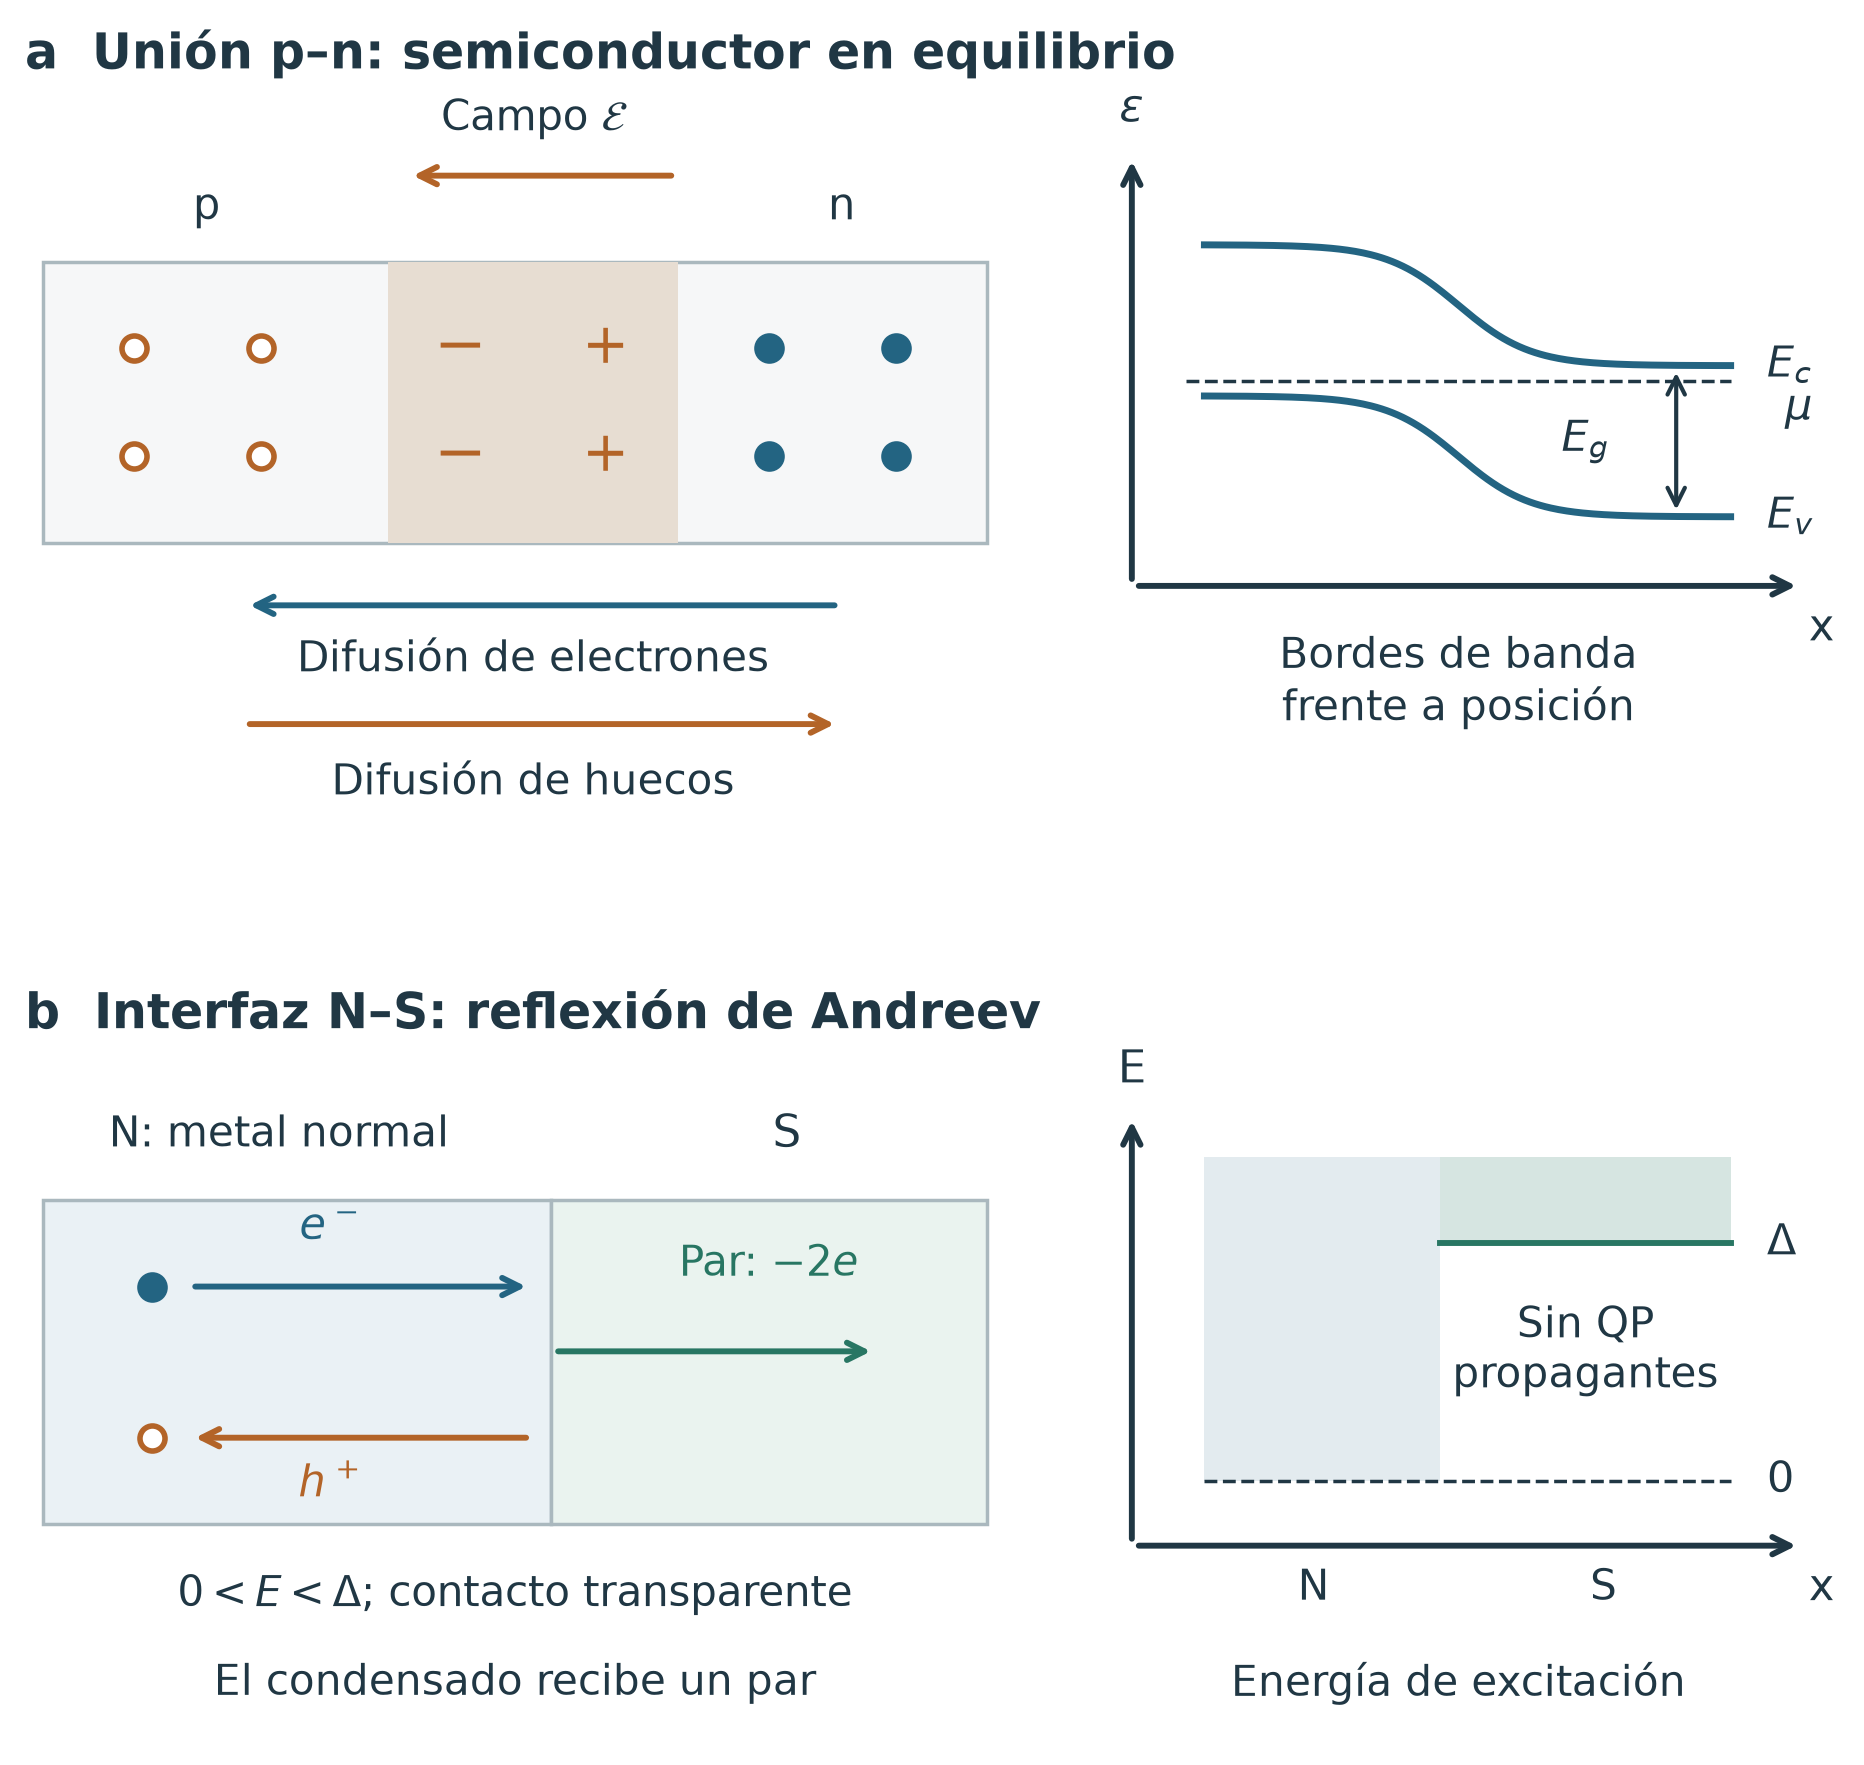
\includegraphics[width=1\linewidth,height=\textheight,keepaspectratio,alt={Figura E.2b. Arriba: unión p--n en equilibrio, con cargas fijas en la región de agotamiento y bordes de banda curvados; las flechas de difusión indican tendencias que la deriva compensa. Abajo: un proceso de reflexión de Andreev en una interfaz transparente entre un metal normal N y un superconductor convencional S. El esquema no identifica el ancho espacial de agotamiento, la barrera electrostática y la brecha superconductora entre sí.}]{../figuras/E04_interfaces.png}
\caption{Figura E.2b. Arriba: unión p--n en equilibrio, con cargas fijas
en la región de agotamiento y bordes de banda curvados; las flechas de
difusión indican tendencias que la deriva compensa. Abajo: un proceso de
reflexión de Andreev en una interfaz transparente entre un metal normal
N y un superconductor convencional S. El esquema no identifica el ancho
espacial de agotamiento, la barrera electrostática y la brecha
superconductora entre sí.}
\end{figure}

En la frontera \textbf{N--S}, N significa \emph{metal en estado normal},
no dopaje tipo n.~Para un contacto transparente, un superconductor
convencional de brecha completa y una excitación incidente con
\(0<E<\Delta\), no hay una QP propagante de esa energía en el interior
de S. Puede reflejarse un hueco hacia N mientras se incorpora al
condensado un par de electrones: \textbf{reflexión de Andreev}. El hueco
es aquí una ausencia en el metal normal, no en una banda de valencia
semiconductora. Si el electrón incidente lleva carga \(-e\) hacia S y el
hueco reflejado lleva \(+e\) hacia N, S recibe carga neta \(-2e\). Se
convierte corriente normal en supercorriente; no se trata de
recombinación p--n.~Una barrera poco transparente favorece también la
reflexión normal; por encima de \(\Delta\) pueden transmitirse QP.
\href{https://harvest.aps.org/v2/journals/articles/10.1103/PhysRevB.25.4515/fulltext}{Blonder,
Tinkham y Klapwijk, interfaz N--S}.

Las dos fronteras permiten usar electrones y huecos para conservar
carga. Lo que cambia es el estado de referencia y el mecanismo de
transporte: redistribución e inyección entre bandas en p--n; intercambio
de pares con un condensado en N--S.

\subsection{E.2.4. Actividad}\label{e.2.4.-actividad}

\Needspace{4\baselineskip}

\textbf{E04.1, 4 puntos.} Añadir un electrón a \(\mu+4\) meV y retirar
otro a \(\mu-1\) meV. Completar por separado \(\delta N\), \(\delta Q\)
y \(\delta E_{\rm exc}\) de cada operación y sus totales.

\textbf{Respuesta E04.1:} \emph{Escribir aquí.}

\Needspace{4\baselineskip}

\textbf{E04.2, 3 puntos.} En la imagen local de una vacante, si ésta va
a la derecha, ¿hacia dónde saltó el electrón y hacia dónde apunta la
corriente convencional asociada a ese salto? Explicar usando su carga.

\textbf{Respuesta E04.2:} \emph{Escribir aquí.}

\Needspace{4\baselineskip}

\textbf{E04.3, 3 puntos.} Corregir: «una población de excitaciones
eléctricamente neutra debe tener energía cero».

\textbf{Respuesta E04.3:} \emph{Escribir aquí.}

\textbf{Condición esencial:} declarar la referencia y conservar los
signos de carga y energía.

Los conteos, velocidades y energías de los ejemplos se han elegido para
comprobar las ideas; no son parámetros del detector.

\Needspace{14\baselineskip}

\bigskip

\section{E.3. Ocupaciones y operadores ---
E06}\label{e.3.-ocupaciones-y-operadores-e06}

\textbf{Revisión: r2. Estado: ABIERTO. Meta:} distinguir un modo
electrónico, su ocupación y las operaciones que cambian esa ocupación.

\subsection{E.3.1. Introducción: elegir qué conviene
seguir}\label{e.3.1.-introducciuxf3n-elegir-quuxe9-conviene-seguir}

Para describir varios electrones interesa saber qué formas de movimiento
están disponibles y cómo se ocupan. Numerar los electrones como si cada
uno tuviera una identidad observable añade un seguimiento que su
indistinguibilidad no permite. La \textbf{representación de
ocupaciones}, llamada segunda cuantización, organiza la descripción por
modos: especifica cuáles están vacíos, cuáles ocupados y qué operaciones
transfieren ocupaciones entre ellos. Las posiciones y los momentos
siguen teniendo significado físico; ahora su información está en los
modos elegidos y en el estado que los ocupa.

El propósito es comparable al de pasar de fuerzas newtonianas a una
formulación lagrangiana: una elección distinta de objetos matemáticos
puede facilitar un problema y conservar su contenido físico. En la
mecánica clásica, las energías y las coordenadas generalizadas ayudan a
tratar restricciones. En un problema cuántico de muchos electrones, los
modos y sus ocupaciones ayudan a tratar partículas indistinguibles e
intercambios. Esta analogía explica la utilidad de reformular; la
cuantización requiere además la física cuántica.

\subsection{E.3.2. Una comprobación familiar: de Lagrange a
Newton}\label{e.3.2.-una-comprobaciuxf3n-familiar-de-lagrange-a-newton}

Tomemos una masa \(m\) unida a un resorte de constante \(K\). La
coordenada \(x\) es aquí el desplazamiento respecto del equilibrio y
\(\dot x=dx/dt\) es su velocidad. Definimos el lagrangiano como energía
cinética menos energía potencial:

\[
L(x,\dot x)=\frac12m\dot x^2-\frac12Kx^2,
\qquad
\frac{d}{dt}\frac{\partial L}{\partial\dot x}
-\frac{\partial L}{\partial x}=0.
\tag{E06.a}
\]

La segunda expresión es la ecuación de Euler--Lagrange. Al calcular sus
dos derivadas se recupera la fuerza restauradora de Newton:

\[
\frac{\partial L}{\partial\dot x}=m\dot x,
\qquad \frac{\partial L}{\partial x}=-Kx
\quad\Longrightarrow\quad
m\ddot x+Kx=0
\quad\Longrightarrow\quad m\ddot x=-Kx.
\tag{E06.b}
\]

Por ejemplo, con \(m=0.20\) kg, \(K=8.0\) N/m y \(x=0.030\) m, Newton da
\(F=-Kx=-0.24\) N y \(\ddot x=F/m=-1.2\) m/s\(^2\). Euler--Lagrange da
\(\ddot x=-(K/m)x=-1.2\) m/s\(^2\). Se ha reorganizado el cálculo de la
misma aceleración. El paso a ocupaciones buscará una comodidad
semejante, esta vez dentro de una descripción cuántica.

\subsection{E.3.3. Un modo concreto antes de introducir sus
operadores}\label{e.3.3.-un-modo-concreto-antes-de-introducir-sus-operadores}

Elijamos un orbital espacial de la muestra y fijemos el espín arriba
respecto de un eje. El orbital especifica una forma espacial permitida
para el electrón; el espín completa la etiqueta de \textbf{este modo
fermiónico}. «Modo» no identifica un electrón particular ni significa
necesariamente una vibración. El mismo orbital con espín abajo
constituye otro modo.

Para el modo elegido hay dos ocupaciones permitidas: \textbf{0 significa
que no hay un electrón en él; 1 significa que hay uno}. El principio de
exclusión impide una ocupación 2 en ese mismo orbital con ese mismo
espín. El modo disponible es el mismo tanto cuando está vacío como
cuando está ocupado. Por tanto, hay que separar la pregunta «¿qué modo
elegí?» de «¿en qué estado de ocupación se encuentra?».

Representaremos esos dos estados mediante columnas. Los símbolos
\(|0\rangle\) y \(|1\rangle\), llamados \emph{kets}, nombran las
columnas del estado vacío y del ocupado. Después introducimos las
matrices \(c\) y \(c^\dagger\) para retirar y añadir una ocupación:

\[
|0\rangle=\begin{pmatrix}1\\0\end{pmatrix},\quad
|1\rangle=\begin{pmatrix}0\\1\end{pmatrix},\quad
c=\begin{pmatrix}0&1\\0&0\end{pmatrix},\quad
c^\dagger=\begin{pmatrix}0&0\\1&0\end{pmatrix}.
\tag{E.2}
\]

La daga \(\dagger\) significa transponer y conjugar complejamente una
matriz. Aquí las entradas son reales y basta transponer. La primera
entrada de cada columna corresponde a la base «vacío» y la segunda a
«ocupado»; no son coordenadas espaciales. Multiplicar las matrices
permite comprobar sus nombres:

\[
c|1\rangle=|0\rangle,\quad c|0\rangle=0,
\qquad c^\dagger|0\rangle=|1\rangle,\quad c^\dagger|1\rangle=0.
\tag{E.3}
\]

El \(0\) de la derecha es el \textbf{vector cero}, no el ket de vacío
\(|0\rangle\). Retirar de un modo vacío o añadir a uno ya ocupado no
produce un estado permitido mediante esa operación. En cambio, retirar
del ocupado produce un estado físico bien definido: el modo sigue
disponible y queda vacío. Así se cierra el hilo: el orbital y su espín
identifican el modo; el ket indica cómo está ocupado; la matriz cambia
esa ocupación.

\begin{figure}
\centering
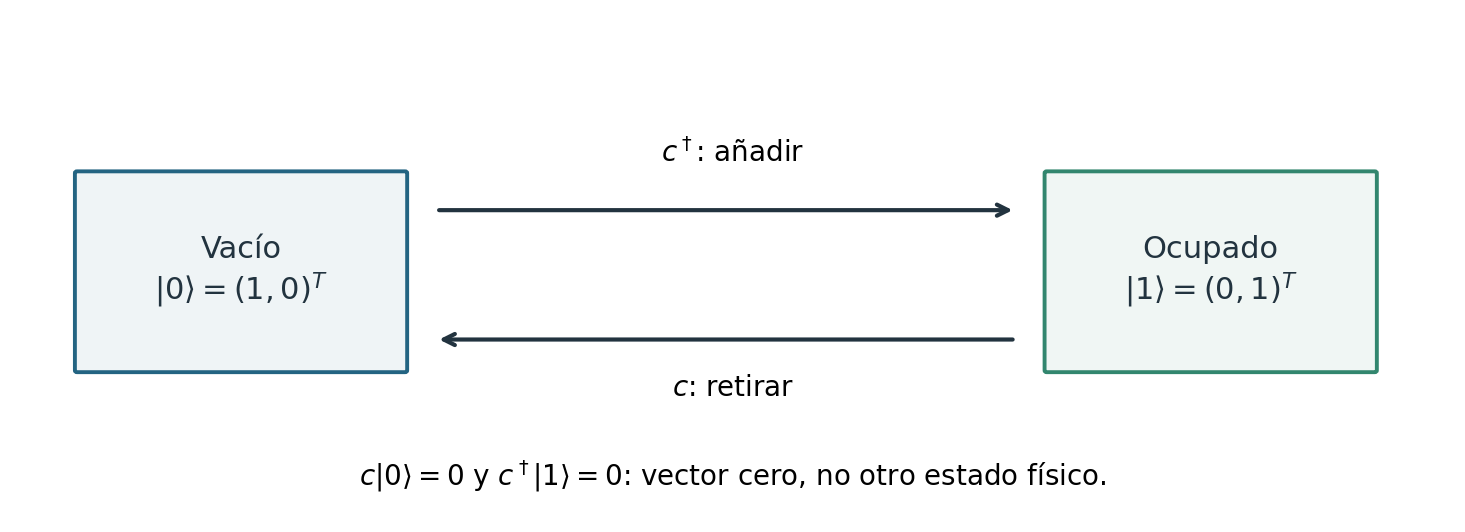
\includegraphics[width=0.97\linewidth,height=\textheight,keepaspectratio,alt={Figura E.3. Acciones de añadir y retirar en un único orbital con espín fijado. «Vacío» es un estado de ocupación y tiene un vector no nulo.}]{../figuras/E06_ocupacion_operadores.png}
\caption{Figura E.3. Acciones de añadir y retirar en un único orbital
con espín fijado. «Vacío» es un estado de ocupación y tiene un vector no
nulo.}
\end{figure}

\subsection{E.3.4. Ejemplo resuelto: contar la
ocupación}\label{e.3.4.-ejemplo-resuelto-contar-la-ocupaciuxf3n}

El operador número \(\hat n\) se define como \(c^\dagger c\). La matriz
de la derecha actúa primero:

\[
\hat n=c^\dagger c=\begin{pmatrix}0&0\\0&1\end{pmatrix},
\qquad \hat n|0\rangle=0,\quad \hat n|1\rangle=|1\rangle.
\tag{E.4}
\]

En el ket ocupado, retirar y reponer da el mismo ket multiplicado por 1.
En el vacío, el resultado se puede escribir \(0|0\rangle\): el valor
contado es 0. Ésta es una composición matemática de operadores; medir la
ocupación no exige retirar físicamente y reponer el electrón.

Al multiplicar en el otro orden se obtiene
\(cc^\dagger=\operatorname{diag}(1,0)\). Por tanto,
\(cc^\dagger+c^\dagger c=I\), donde \(I\) es la identidad. La suma
\(AB+BA\) se llama \textbf{anticomutador}. Su consecuencia concreta es
\(cc^\dagger=I-\hat n\): si \(\hat n\) cuenta la ocupación electrónica
del modo, su complemento cuenta si está vacío.

Con varios modos se usan kets como \(|1,0\rangle\): uno ocupado y otro
vacío, según el orden de etiquetas declarado. Un estado cuántico también
puede ser una superposición de configuraciones; por ejemplo,
\(\bigl(|1,0\rangle+|0,1\rangle\bigr)/\sqrt2\) tiene un electrón total y
no asigna una ocupación definida a cada modo por separado. Por eso la
lista de modos disponibles tampoco basta para especificar el estado de
muchos electrones. Al operar con varios modos fermiónicos hay que
respetar además sus reglas de signos; las matrices de dos entradas
usadas aquí describen sólo un modo.

\subsection{E.3.5. Actividad}\label{e.3.5.-actividad}

\Needspace{4\baselineskip}

\textbf{E06.1, 4 puntos.} Multiplicar explícitamente
\(c^\dagger c|1\rangle\) y \(cc^\dagger|1\rangle\). Indicar en qué paso
importa el orden.

\textbf{Respuesta E06.1:} \emph{Escribir aquí.}

\Needspace{4\baselineskip}

\textbf{E06.2, 3 puntos.} Explicar la diferencia entre el ket
\(|0\rangle\) y el vector cero de E.3.

\textbf{Respuesta E06.2:} \emph{Escribir aquí.}

\Needspace{4\baselineskip}

\textbf{E06.3, 3 puntos.} Hay dos modos distintos, uno de espín arriba y
otro abajo, con el mismo orbital espacial. ¿La prohibición de dos
fermiones en el mismo modo impide ocupar uno en cada modo? Identificar
qué etiqueta cambió.

\textbf{Respuesta E06.3:} \emph{Escribir aquí.}

\textbf{Condición esencial:} distinguir modo, estado de ocupación,
operador y resultado de una operación.

\textbf{Utilidad para el modelo:} las operaciones de añadir y retirar
permiten escribir transferencia electrónica y emparejamiento. Las
ocupaciones medias que entran en balances son números obtenidos del
estado; no son las matrices \(c\).

\textbf{Fuentes:}
\href{https://ocw.mit.edu/courses/8-09-classical-mechanics-iii-fall-2014/d9bac33f6c60b304dc0398e99b327102_MIT8_09F14_full.pdf}{MIT
8.09, notas de Iain Stewart, sección 1.2}, para la equivalencia
mecánica;
\href{https://www.tkm.kit.edu/downloads/ss2016_tkm2/second_quantization.pdf}{KIT,
Second Quantization, sección de fermiones}, para modos, ocupaciones y
operadores. Los productos de matrices y los números de esta clase se
desarrollan aquí.

\Needspace{14\baselineskip}

\bigskip

\section{E.4. Por qué se usa una columna de Nambu ---
E07}\label{e.4.-por-quuxe9-se-usa-una-columna-de-nambu-e07}

\textbf{Revisión: r2. Estado: ABIERTO. Meta:} entender el motivo de
juntar una operación de retirar con otra de añadir, y distinguir esa
columna de un estado de ocupación.

\subsection{E.4.1. Introducción: el emparejamiento mezcla
operaciones}\label{e.4.1.-introducciuxf3n-el-emparejamiento-mezcla-operaciones}

Un modo electrónico queda identificado por su forma espacial y las demás
etiquetas necesarias, incluido el espín. Su ocupación dice si hay un
electrón en él. Aquí elegimos dos modos relacionados: por ejemplo, uno
de momento \(\mathbf k\) y espín arriba y otro de momento \(-\mathbf k\)
y espín abajo. Se los etiqueta 1 y 2; los operadores \(c_1\) y \(c_2\)
retiran una ocupación de cada modo, mientras \(c_1^\dagger\) y
\(c_2^\dagger\) la añaden.

En una descripción efectiva del emparejamiento superconductor aparecen
términos \(\Delta c_1^\dagger c_2^\dagger\) y \(\Delta^*c_2c_1\): el
primero añade una pareja al sector descrito y el segundo la retira. El
orden escrito fija la convención del ejemplo. El número complejo
\(\Delta\) tiene unidades de energía y representa el emparejamiento; su
conjugado \(\Delta^*\) acompaña al proceso inverso para que el operador
de energía sea hermítico. El condensado actúa como referencia colectiva
de esos intercambios. El sistema completo conserva la carga.

La energía normal de cada modo, medida desde el potencial químico, se
llama \(\xi\); se supone igual para esta pareja. Para organizar los
términos normales y de emparejamiento, se define la \textbf{columna de
operadores de Nambu}

\[
\Psi=\begin{pmatrix}c_1\\c_2^\dagger\end{pmatrix},\qquad
H_{\rm BdG}=\begin{pmatrix}\xi&\Delta\\\Delta^*&-\xi\end{pmatrix}.
\tag{E.5}
\]

BdG abrevia Bogoliubov--de Gennes. \(H_{\rm BdG}\) es una matriz de
coeficientes de energía. \textbf{\(\Psi\) contiene operaciones sobre
estados; no es un ket ni una lista de dos electrones adicionales.} Sus
entradas reúnen dos procesos que el emparejamiento relaciona. La
siguiente expansión permite comprobar por qué esa organización resulta
útil.

\begin{figure}
\centering
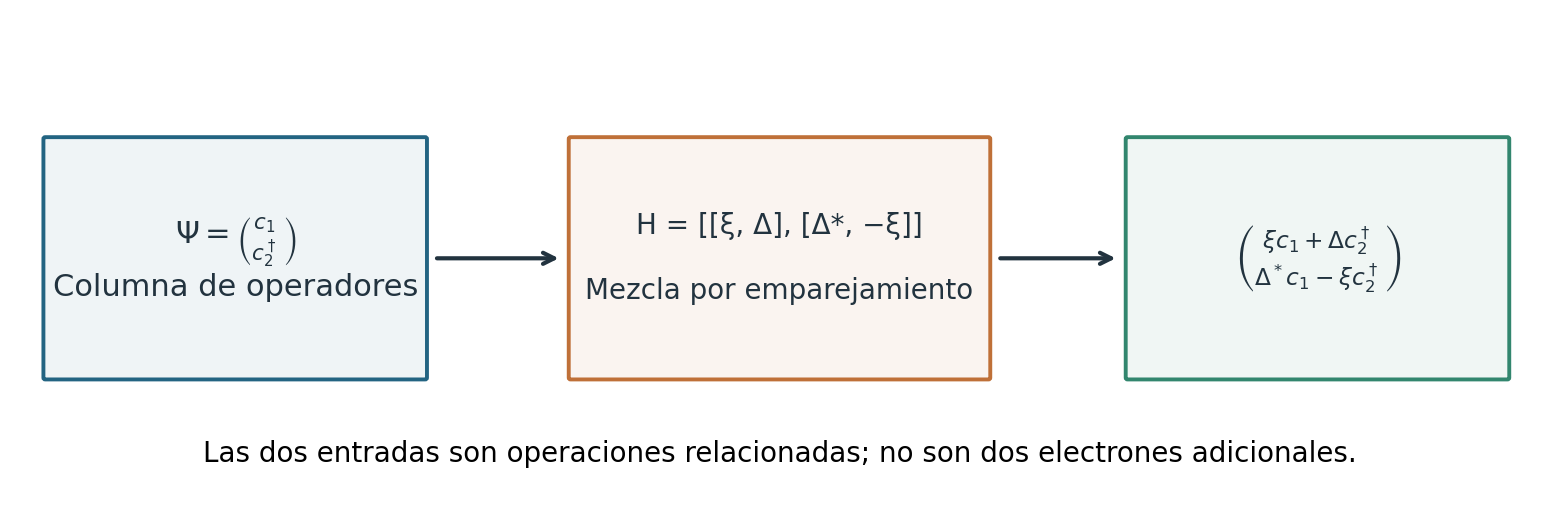
\includegraphics[width=1\linewidth,height=\textheight,keepaspectratio,alt={Figura E.4. Multiplicar una matriz por una columna de operadores combina operaciones de retirar y añadir. El emparejamiento aparece fuera de la diagonal.}]{../figuras/E07_columna_nambu.png}
\caption{Figura E.4. Multiplicar una matriz por una columna de
operadores combina operaciones de retirar y añadir. El emparejamiento
aparece fuera de la diagonal.}
\end{figure}

\subsection{E.4.2. Ejemplo resuelto: de la matriz al contenido
físico}\label{e.4.2.-ejemplo-resuelto-de-la-matriz-al-contenido-fuxedsico}

Para esta pareja de modos, sin sumar otra vez el bloque equivalente,
multiplicar fila, matriz y columna da

\[
\begin{aligned}
\Psi^\dagger H_{\rm BdG}\Psi
={}&\xi c_1^\dagger c_1-\xi c_2c_2^\dagger
+\Delta c_1^\dagger c_2^\dagger+\Delta^*c_2c_1\\
={}&\xi(\hat n_1+\hat n_2-1)
+\Delta c_1^\dagger c_2^\dagger+\Delta^*c_2c_1.
\end{aligned}\tag{E.6}
\]

La segunda línea usa \(\hat n_i=c_i^\dagger c_i\) y la identidad
fermiónica \(c_2c_2^\dagger=1-\hat n_2\). El signo negativo de la
diagonal no asigna al segundo electrón energía normal \(-\xi\): aparece
al colocar creación en esa entrada. Sumando la constante \(\xi\) se
obtiene la energía normal \(\xi(\hat n_1+\hat n_2)\) más los términos
que añaden y retiran parejas.

\Needspace{7\baselineskip}

Con \(\xi=2\) meV y \(\Delta=1\) meV, los valores propios se obtienen de

\[
\det(H_{\rm BdG}-EI)
=E^2-\bigl(2\ {\rm meV}\bigr)^2-\bigl(1\ {\rm meV}\bigr)^2=0,
\qquad E=\pm\sqrt5\ {\rm meV}.
\tag{E.7}
\]

Las operaciones que describen las excitaciones de energía definida son
combinaciones de retirar y añadir, con coeficientes fijados por esta
matriz. Esa combinación es el contenido electrón--hueco de una
cuasipartícula superconductora: retirar un electrón crea una vacante
respecto de la referencia ocupada. Su ocupación indica si esa excitación
está presente; tampoco es una entrada de \(\Psi\).

Las ramas de energía positiva y negativa de la representación BdG están
relacionadas por su construcción electrón--hueco. No se cuentan como dos
especies elementales independientes ni como una duplicación de
electrones físicos. Para este ejemplo basta haber identificado los dos
modos electrónicos, las operaciones sobre ellos y la matriz que las
combina; cada objeto responde a una pregunta distinta.

\subsection{E.4.3. Actividad}\label{e.4.3.-actividad}

\Needspace{4\baselineskip}

\textbf{E07.1, 4 puntos.} Poner \(\Delta=0\) en E.6 y usar la constante
\(+\xi\). Mostrar que quedan las energías normales de los dos modos con
el mismo signo \(+\xi\).

\textbf{Respuesta E07.1:} \emph{Escribir aquí.}

\Needspace{4\baselineskip}

\textbf{E07.2, 3 puntos.} Señalar en E.5 qué entrada describe retirar
una ocupación y cuál añadirla. Explicar por qué ninguna entrada es una
probabilidad de ocupación \(f(E)\).

\textbf{Respuesta E07.2:} \emph{Escribir aquí.}

\Needspace{4\baselineskip}

\textbf{E07.3, 3 puntos.} Corregir: «los dos signos de E.7 demuestran
que aparecieron dos tipos nuevos de partículas elementales».

\textbf{Respuesta E07.3:} \emph{Escribir aquí.}

\textbf{Condición esencial:} explicar el origen de la columna y el signo
diagonal mediante el producto, sin duplicar electrones físicos.

\textbf{Utilidad para el modelo:} la representación organiza el
emparejamiento y el espectro de excitaciones, que luego permiten
calcular ocupaciones, energía y respuesta eléctrica. Aquí se escogió un
bloque de pareja concreto; el factor \(1/2\) de una representación
completa duplicada no se traslada automáticamente a este bloque.

\textbf{Fuente:} \href{https://topocondmat.org/w1-topointro/d/}{TU
Delft, Hamiltoniano BdG y redundancia electrón--hueco}. La expansión y
el ejemplo de energías se calculan aquí.

\Needspace{14\baselineskip}

\bigskip

\section{E.5. Qué significa variar una energía funcional ---
E03}\label{e.5.-quuxe9-significa-variar-una-energuxeda-funcional-e03}

\textbf{Revisión: r2. Estado: ABIERTO. Meta:} reconstruir una primera
variación y entender qué cambia al eliminar una variable interna
estacionaria. No se exige resolver un problema completo de estabilidad
ni calcular segundas variaciones.

\subsection{E.5.1. Introducción: construir primero una curva
ordinaria}\label{e.5.1.-introducciuxf3n-construir-primero-una-curva-ordinaria}

En el ejemplo más sencillo, una función \(F(y)\) recibe un número. Un
funcional \(\mathcal F[y]\) recibe un perfil completo \(y(x)\) y
devuelve un número, por ejemplo una energía. Los corchetes sólo
recuerdan qué tipo de entrada se utiliza. La coordenada \(x\) recorre el
espacio; no representa tiempo en esta clase.

Variar la energía significa comparar cuánto vale \textbf{la misma regla
de energía} para perfiles vecinos del mismo sistema. Se deforma su
configuración; no se cambia arbitrariamente la fórmula ni se exige que
esos perfiles sean una evolución temporal real.

Se elige otro perfil \(\eta(x)\), llamado \textbf{dirección de
perturbación}, y un número pequeño \(\epsilon\) que fija su tamaño.
Tomaremos \(\epsilon\) adimensional y \(\eta\) con las mismas unidades
que \(y\). El perfil ensayado es \(y_\epsilon(x)=y(x)+\epsilon\eta(x)\).
Una vez fijados \(y\) y \(\eta\), evaluar su energía produce la función
ordinaria \(J(\epsilon)=\mathcal F[y_\epsilon]\) de una sola variable.

\begin{figure}
\centering
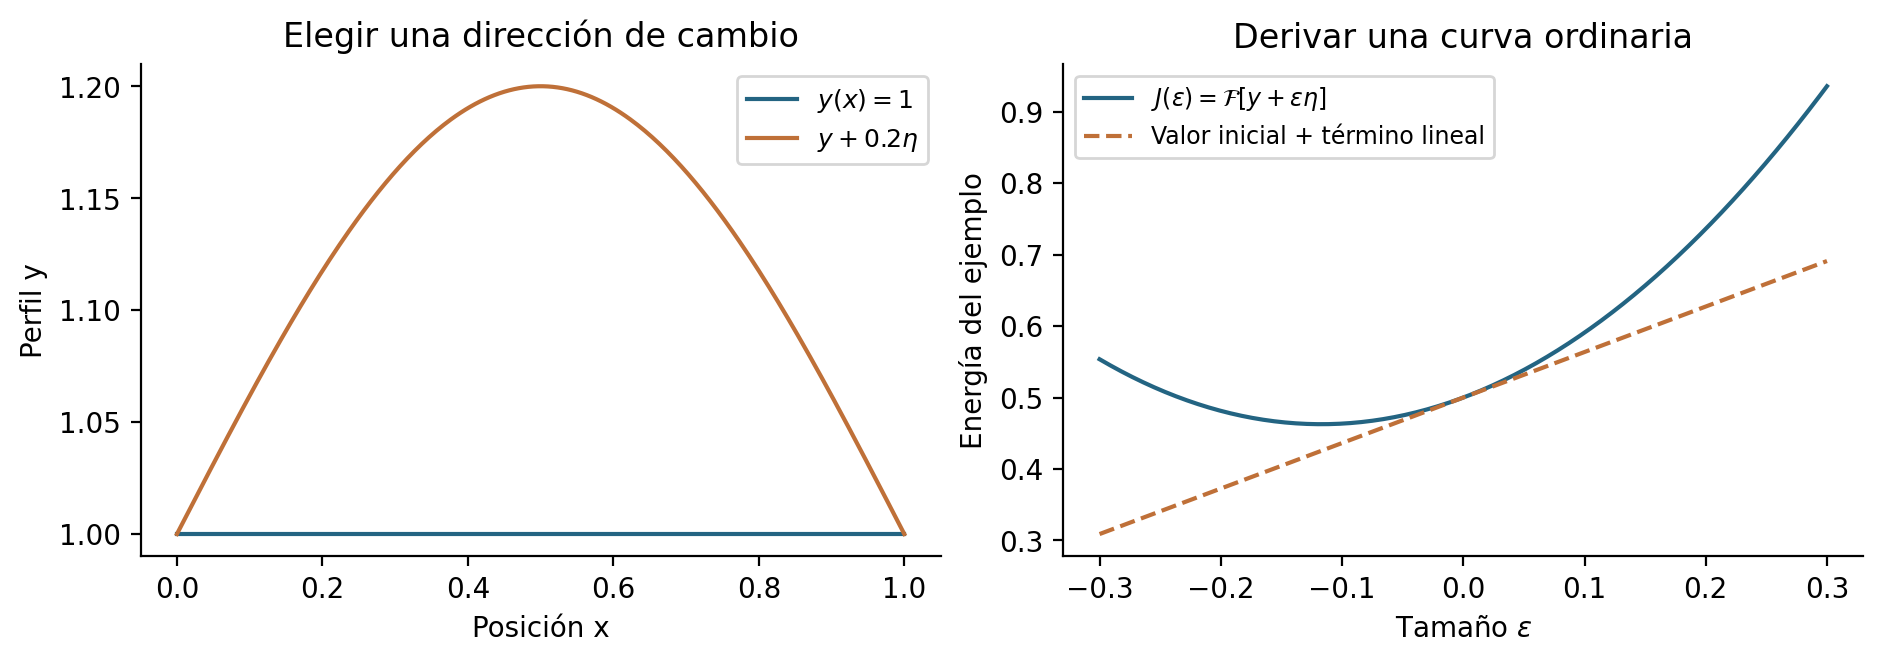
\includegraphics[width=0.96\linewidth,height=\textheight,keepaspectratio,alt={Figura E.5. La variación se convierte en la pendiente de una curva ordinaria. En el ejemplo dibujado, el término cuadrático explica por qué la recta tangente y la curva se separan al alejarse de cero.}]{../figuras/E03_curva_variacion.png}
\caption{Figura E.5. La variación se convierte en la pendiente de una
curva ordinaria. En el ejemplo dibujado, el término cuadrático explica
por qué la recta tangente y la curva se separan al alejarse de cero.}
\end{figure}

La derivada direccional de Gâteaux, también llamada primera variación en
esta aplicación, es

\[
D\mathcal F[y](\eta)
\equiv J'(0)
=\lim_{\epsilon\to0}
\frac{\mathcal F[y+\epsilon\eta]-\mathcal F[y]}{\epsilon}.
\tag{E.8}
\]

La notación se lee en dos pasos: \(D\mathcal F[y]\) es la regla de
respuesta lineal calculada \textbf{en el perfil base} \(y\); \((\eta)\)
indica que esa regla se aplica \textbf{al perfil de perturbación
completo} \(\eta\). Los paréntesis admiten funciones como argumentos: no
convierten a \(\eta\) en una coordenada espacial. En \(\eta(x)\) sí se
evalúa el perfil en un punto \(x\). Aquí se deriva respecto de
\(\epsilon\), manteniendo fijos ambos perfiles. El resultado
\(D\mathcal F[y](\eta)=J'(0)\) es un número, la pendiente de la energía
en esa dirección.

Una versión con dos coordenadas aclara el papel de cada objeto. Si
\(U(\mathbf q)=(q_1^2+q_2^2)/2\), entonces

\[
DU[\mathbf q](\mathbf v)
=\left.\frac{d}{d\epsilon}U(\mathbf q+\epsilon\mathbf v)\right|_0
=q_1v_1+q_2v_2.
\tag{E03.a}
\]

Para \(\mathbf q=(1,2)\) y \(\mathbf v=(3,-1)\) la pendiente es
\(3-2=1\). \(\mathbf v\) es el vector que elegimos para deformar la
configuración, no el escalar respecto del cual derivamos. Al pasar de
dos coordenadas a un perfil, la suma se convierte en una integral.
Cuando, después de tratar los bordes, se puede escribir
\(D\mathcal F[y](\eta)=\int g(x)\eta(x)dx\), llamamos a \(g(x)\)
\textbf{derivada funcional}, escrita \(\delta\mathcal F/\delta y(x)\).
Esta función local y la pendiente integrada son objetos distintos.

\subsection{E.5.2. Ejemplo resuelto: por qué quedan esos
términos}\label{e.5.2.-ejemplo-resuelto-por-quuxe9-quedan-esos-tuxe9rminos}

Se usa una energía adimensional sobre \(0\leq x\leq1\):

\[
\mathcal F[y]=\frac12\int_0^1[(y')^2+y^2]dx,
\qquad y'=\frac{dy}{dx}.
\tag{E.9}
\]

El primer cuadrado penaliza diferencias espaciales; el segundo, la
amplitud del perfil. Para hacer la variación se sustituye \textbf{en
ambos} cuadrados. Como \(\epsilon\) no depende de \(x\),
\((y+\epsilon\eta)'=y'+\epsilon\eta'\). La identidad
\((a+b)^2=a^2+2ab+b^2\) da exactamente

\[
\mathcal F[y+\epsilon\eta]-\mathcal F[y]
=\epsilon\int_0^1(y'\eta'+y\eta)dx
+\frac{\epsilon^2}{2}\int_0^1[(\eta')^2+\eta^2]dx.
\tag{E.10}
\]

No se ha descartado nada. Al dividir por \(\epsilon\), el primer término
ya no depende de él y el segundo conserva un factor \(\epsilon\). El
límite de E.8 elimina ese segundo término. Se retienen los términos
lineales \textbf{porque se está calculando una derivada en cero}, no
porque los demás sean físicamente inexistentes.

Para reemplazar \(\eta'\) por \(\eta\) se utiliza integración por
partes, que viene de integrar la regla del producto
\((y'\eta)'=y''\eta+y'\eta'\):

\[
D\mathcal F[y](\eta)
=[y'\eta]_0^1+\int_0^1(-y''+y)\eta\,dx.
\tag{E.11}
\]

Fijar los extremos significa exigir los \textbf{mismos valores} \(y_0\)
y \(y_1\) a todos los perfiles que comparamos. Esos valores pueden
elegirse arbitrariamente al plantear el problema; una vez elegidos, no
varían con \(\epsilon\). Como \(y(0)=y_0\) y \(y(1)=y_1\), se exige

\[
\begin{aligned}
y_\epsilon(0)=y_0+\epsilon\eta(0)=y_0
&\ \Longrightarrow\ \epsilon\eta(0)=0,\\
y_\epsilon(1)=y_1+\epsilon\eta(1)=y_1
&\ \Longrightarrow\ \epsilon\eta(1)=0.
\end{aligned}\tag{E03.b}
\]

Estas igualdades deben valer para todo \(\epsilon\) suficientemente
pequeño, incluidos valores no nulos. Por eso \(\eta(0)=\eta(1)=0\)
aunque \(y_0\) e \(y_1\) no sean cero. Por ejemplo, una cuerda con
extremos en alturas 2 y 5 puede ensayarse con \(y(x)=2+3x\) y
\(\eta(x)=\sin(\pi x)\): la deformación cambia el interior y conserva
ambas alturas. Con esa condición desaparece el término de borde y se
identifica \(\delta\mathcal F/\delta y=-y''+y\). Si los extremos pueden
moverse, ese término informa del trabajo de borde y se conserva hasta
especificar qué otra condición corresponde.

\textbf{Comprobación numérica del dibujo.} Para \(y=1\) y
\(\eta=\sin(\pi x)\), se obtiene \(D\mathcal F[y](\eta)=2/\pi\). La
curva exacta es \(J(\epsilon)=1/2+2\epsilon/\pi+(\pi^2+1)\epsilon^2/4\).
Su pendiente en cero vuelve a ser \(2/\pi\). El script verifica esa
pendiente con diferencias centrales.

\subsection{E.5.3. La envolvente, con una sola regla de la
cadena}\label{e.5.3.-la-envolvente-con-una-sola-regla-de-la-cadena}

Algunos modelos contienen variables internas que ya satisfacen su
condición estacionaria. Para ver qué cambia al eliminarlas, usar
\(F(y,z)=y^2/2+(z-2y)^2/2\), donde \(y,z\) son ahora números, no
perfiles. La variable interna estacionaria satisface \(F_z=z-2y=0\), así
que \(z^*(y)=2y\). Definir \(\bar F(y)=F(y,z^*(y))\) y aplicar la regla
de la cadena:

\[
\frac{d\bar F}{dy}=F_y+F_z\frac{dz^*}{dy}=F_y,
\qquad F_z(y,z^*(y))=0.
\tag{E.12}
\]

Ésta es la forma estacionaria del \textbf{teorema de la envolvente},
para una rama diferenciable. La derivada interna no se elimina porque
\(z^*\) sea constante, sino porque multiplica una pendiente cero. Aquí
\(\bar F=y^2/2\) y la derivada vale \(y\). En un modelo con varias
variables, resolver una variable interna no obliga a que las restantes
estén también en equilibrio. Este paso y E.11 son el objetivo de la
clase; el análisis de curvaturas puede esperar.

\subsection{E.5.4. Actividad}\label{e.5.4.-actividad}

\Needspace{4\baselineskip}

\textbf{E03.1, 4 puntos.} Para
\(\mathcal G[y]=\frac12\int_0^1 y(x)^2dx\), expandir
\(\mathcal G[y+\epsilon\eta]-\mathcal G[y]\), dividir por \(\epsilon\) y
tomar el límite. No hay derivadas espaciales en este ejercicio.

\textbf{Respuesta E03.1:} \emph{Escribir aquí.}

\Needspace{4\baselineskip}

\textbf{E03.2, 3 puntos.} En E.11, explicar qué condición permite quitar
\([y'\eta]_0^1\). ¿Basta con decir «se integra sobre todo el dominio»?

\textbf{Respuesta E03.2:} \emph{Escribir aquí.}

\Needspace{4\baselineskip}

\textbf{E03.3, 3 puntos.} En E.12, indicar cuál factor vale cero y
explicar por qué eso no implica \(d\bar F/dy=0\).

\textbf{Respuesta E03.3:} \emph{Escribir aquí.}

\textbf{Condición esencial:} identificar perfil, dirección, tamaño y
pendiente, y justificar el término de borde. Fuente para nombre y
definición:
\href{https://ocw.mit.edu/courses/18-325-topics-in-applied-mathematics-waves-and-imaging-fall-2015/834e98a77f64597a422c205b123cd6d7_MIT18_325F15_Appendix_A.pdf}{MIT
18.325, cálculo de variaciones, apéndice A}. Las expansiones y el
ejemplo de envolvente se calculan aquí.

\Needspace{14\baselineskip}

\bigskip

\section{E.6. De dos masas a una distribución de modos ---
E05}\label{e.6.-de-dos-masas-a-una-distribuciuxf3n-de-modos-e05}

\textbf{Revisión: r2. Estado: ABIERTO. Meta:} separar forma de
vibración, frecuencia, distribución de modos, ocupación y energía.

\subsection{E.6.1. Introducción desde modos
normales}\label{e.6.1.-introducciuxf3n-desde-modos-normales}

El sistema será dos masas iguales \(m\) que pueden desplazarse a lo
largo de una línea. Sus desplazamientos respecto del equilibrio son
\(u_1,u_2\); tres resortes de constante \(K\) las conectan entre sí y a
paredes fijas. Hay dos coordenadas independientes y, en esta
aproximación lineal estable, dos modos normales. Un \textbf{modo normal}
es un patrón de desplazamientos que puede oscilar con una frecuencia
propia. El movimiento general combina ambos patrones con amplitudes y
fases que dependen de cómo se preparó el sistema.

Si aumentamos el número de masas, enumerar cada frecuencia puede
volverse poco práctico. Entonces preguntamos cuántos modos caen en cada
intervalo de frecuencias. Esa organización es una \textbf{distribución
de modos}. La densidad de estados, abreviada DOS por \emph{density of
states}, expresa ese conteo por unidad de intervalo. Primero
construiremos el conteo clásico; después distinguiremos la cuantización
de la energía de cada modo. Encontrar frecuencias permitidas mediante
paredes y resortes no basta para cuantizar sus amplitudes o energías.

\begin{figure}
\centering
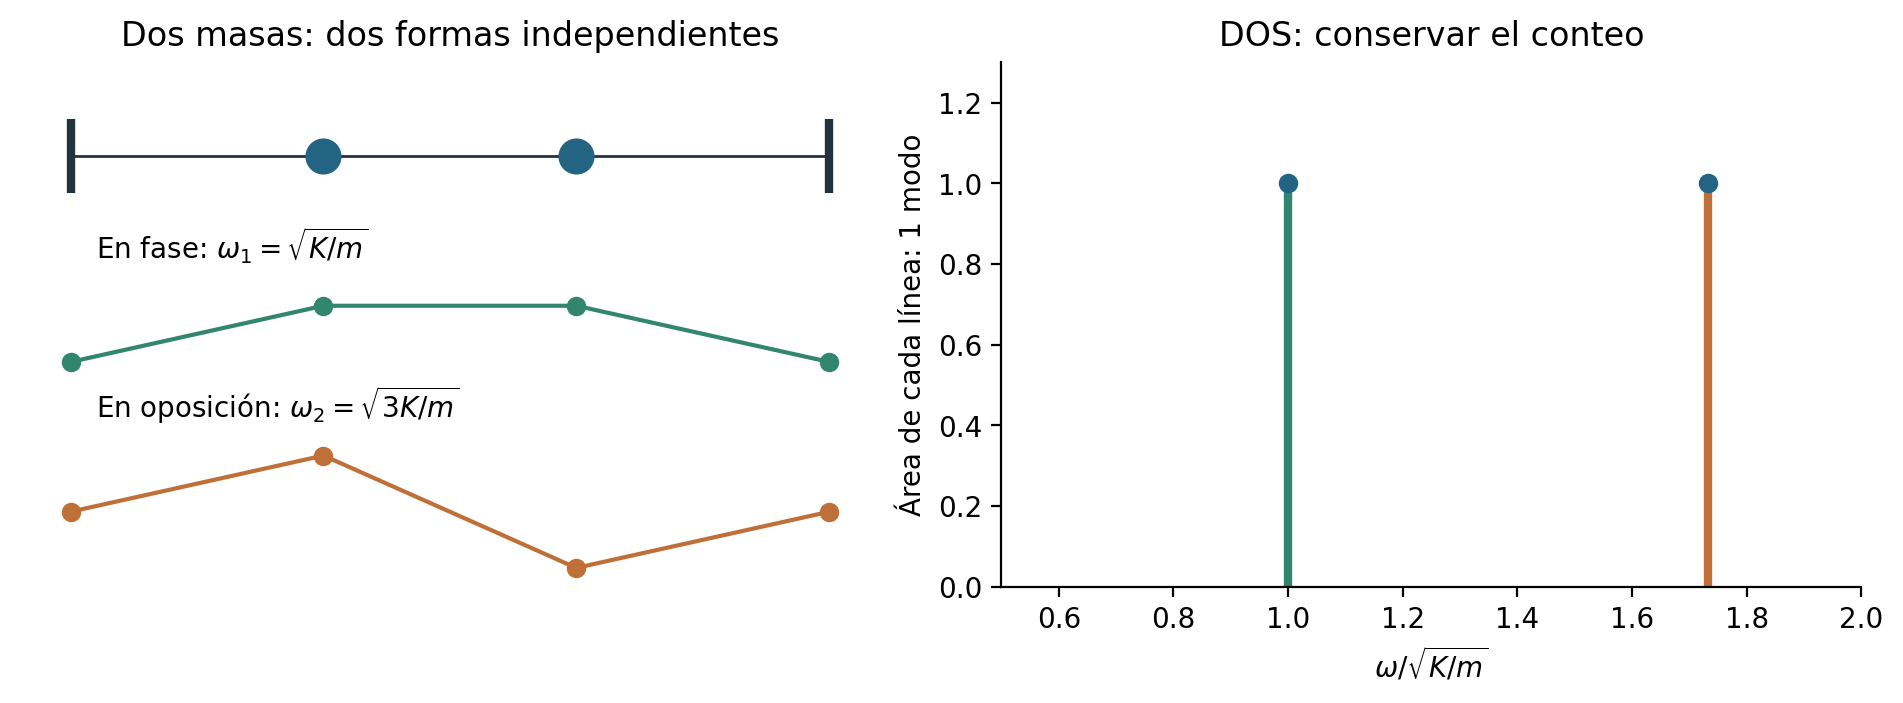
\includegraphics[width=0.98\linewidth,height=\textheight,keepaspectratio,alt={Figura E.6. Dos patrones independientes y sus frecuencias. Las líneas de la derecha representan el peso de un modo cada una; no indican la amplitud de vibración ni el número de fonones presentes.}]{../figuras/E05_modos_conteo.png}
\caption{Figura E.6. Dos patrones independientes y sus frecuencias. Las
líneas de la derecha representan el peso de un modo cada una; no indican
la amplitud de vibración ni el número de fonones presentes.}
\end{figure}

\subsection{E.6.2. Ejemplo resuelto: de fuerzas a
frecuencias}\label{e.6.2.-ejemplo-resuelto-de-fuerzas-a-frecuencias}

La energía potencial suma el alargamiento al cuadrado de cada resorte:

\[
V=\frac K2[u_1^2+(u_2-u_1)^2+u_2^2],\qquad
m\ddot{\mathbf u}=-K\begin{pmatrix}2&-1\\-1&2\end{pmatrix}\mathbf u.
\tag{E.13}
\]

\(\mathbf u=(u_1,u_2)^T\) es la columna de desplazamientos; los puntos
indican derivadas temporales. La matriz aparece al calcular las fuerzas
\(-\partial V/\partial u_i\). Ensayar
\(\mathbf u(t)=\mathbf v\cos(\omega t)\) transforma la ecuación de
movimiento en un problema de valores propios. Los vectores
\(\mathbf v_1=(1,1)^T/\sqrt2\) y \(\mathbf v_2=(1,-1)^T/\sqrt2\)
describen movimiento en fase y en oposición. Sus valores propios
adimensionales son 1 y 3:

\[
\omega_1=\sqrt{K/m},\qquad \omega_2=\sqrt{3K/m}.
\tag{E.14}
\]

La frecuencia angular \(\omega\) se mide en rad/s. Con \(K=1\) N/m y
\(m=1\) kg obtenemos \(\omega_1=1\) rad/s y \(\omega_2\simeq1.732\)
rad/s. Ambos modos existen aunque las masas se encuentren en reposo.

\subsection{E.6.3. Qué distribuye una
DOS}\label{e.6.3.-quuxe9-distribuye-una-dos}

Para los números anteriores podemos agrupar frecuencias en dos
intervalos. La altura del histograma se calcula dividiendo el conteo por
el ancho:

{\def\LTcaptype{none} % do not increment counter
\begin{longtable}[]{@{}
  >{\raggedright\arraybackslash}p{(\linewidth - 6\tabcolsep) * \real{0.2500}}
  >{\raggedleft\arraybackslash}p{(\linewidth - 6\tabcolsep) * \real{0.2500}}
  >{\raggedleft\arraybackslash}p{(\linewidth - 6\tabcolsep) * \real{0.2500}}
  >{\raggedleft\arraybackslash}p{(\linewidth - 6\tabcolsep) * \real{0.2500}}@{}}
\toprule\noalign{}
\begin{minipage}[b]{\linewidth}\raggedright
Intervalo de \(\omega\), en rad/s
\end{minipage} & \begin{minipage}[b]{\linewidth}\raggedleft
Modos en el intervalo
\end{minipage} & \begin{minipage}[b]{\linewidth}\raggedleft
Ancho, en rad/s
\end{minipage} & \begin{minipage}[b]{\linewidth}\raggedleft
Altura: modos por rad/s
\end{minipage} \\
\midrule\noalign{}
\endhead
\bottomrule\noalign{}
\endlastfoot
\([0,1.5)\) & 1 & 1.5 & \(2/3\) \\
\([1.5,2.0)\) & 1 & 0.5 & 2 \\
\end{longtable}
}

El segundo rectángulo es tres veces más alto y contiene exactamente el
mismo número de modos. Su área es \(2\times0.5=1\), mientras la del
primero es \((2/3)\times1.5=1\). La integral del histograma vale 2. Así,
\textbf{distribuir significa registrar dónde se encuentra lo contado;
densidad significa dividir ese conteo por el tamaño del intervalo}. Al
cambiar los intervalos cambia la apariencia del histograma, pero se
conserva el total.

Para guardar exactamente las dos frecuencias, sin agruparlas, se escribe

\[
F_\omega(\omega)=\delta(\omega-\omega_1)+\delta(\omega-\omega_2),
\qquad \int_0^\infty F_\omega(\omega)d\omega=2.
\tag{E.15}
\]

La delta de Dirac es una \textbf{distribución en sentido matemático}: se
define por su acción dentro de una integral, no como una función
ordinaria a la que debamos asignar una altura infinita. Para cualquier
función suave \(a(\omega)\),

\[
\int_0^\infty a(\omega)\,
\delta(\omega-\omega_j)d\omega=a(\omega_j),
\qquad \omega_j>0.
\tag{E05.a}
\]

Con \(a=1\), cada delta aporta uno al conteo; con otro peso, selecciona
el valor de ese peso en la frecuencia del modo. En una figura se dibujan
líneas de peso uno o picos ensanchados de área uno. La altura aislada no
es el objeto físico. Una curva suave de DOS aproxima muchas frecuencias
cercanas, o incorpora un ensanchamiento declarado.

Esta distribución de modos tampoco es por sí sola una distribución de
probabilidad. Si se eligiera al azar uno de estos dos modos, con igual
probabilidad, \(p_\omega=F_\omega/2\) sería una distribución normalizada
a 1. Ese experimento de selección es una pregunta adicional. La DOS
original cuenta 2 modos, aunque ninguno esté excitado.

\subsection{E.6.4. Cuándo aparece el cuanto de
energía}\label{e.6.4.-cuuxe1ndo-aparece-el-cuanto-de-energuxeda}

La mecánica de Newton o de Lagrange permite que la amplitud y la energía
de un oscilador clásico varíen continuamente. Históricamente, la
discontinuidad no se dedujo sólo de cambiar la formulación mecánica.
Planck introdujo en 1900 elementos de energía proporcionales a la
frecuencia para contar las maneras de repartir energía entre resonadores
y explicar la radiación térmica. Einstein aplicó en 1907 esa idea a
osciladores de un sólido para explicar su calor específico. Son pasos
físicos adicionales, motivados por fenómenos que la descripción clásica
no explicaba. Véanse las fuentes originales al final de la clase.

En la mecánica cuántica, cada modo armónico independiente tiene niveles

\[
E_{n,j}=\left(n+\frac12\right)\hbar\omega_j,
\qquad n=0,1,2,\ldots,
\qquad E_{n+1,j}-E_{n,j}=\hbar\omega_j=h\nu_j.
\tag{E05.b}
\]

\(h\) es la constante de Planck, \(\hbar=h/(2\pi)\) y
\(\nu=\omega/(2\pi)\) es la frecuencia ordinaria en ciclos por segundo.
Un \textbf{fonón} es un cuanto de excitación de un modo vibracional del
sólido. La ocupación \(n_j\) cuenta esos cuantos; el término
\(\hbar\omega_j/2\) es la energía de punto cero, presente incluso con
\(n_j=0\).

Con \(n_1=2\) y \(n_2=0\), hay dos modos disponibles y dos cuantos,
ambos en el primero. La energía de excitación, medida respecto del
estado con todos los modos en \(n_j=0\), es \(2\hbar\omega_1\). Si ahora
\(n_1=4\), la energía de excitación se duplica y el conteo de modos
sigue siendo 2. La DOS indica \textbf{dónde puede alojarse} energía; las
ocupaciones indican \textbf{cuánta se ha alojado}.

Si la ocupación fluctúa, definimos \(P_j(n)\) como la probabilidad de
medir \(n\) cuantos y \(\bar n_j=\sum_{n=0}^\infty nP_j(n)\) como su
promedio. Por ejemplo, \(P(0)=P(1)=1/2\) da \(\bar n=1/2\): cada
medición cuenta 0 o 1, y el promedio de muchas mediciones es 0.5. No se
ha creado medio fonón en un estado de número definido. Para modos
independientes, la energía media de excitación es
\(\sum_j\hbar\omega_j\bar n_j\).

La cuantización también puede observarse en un modo colectivo de un
objeto formado por muchos átomos: O'Connell y colaboradores prepararon y
controlaron excitaciones de un fonón en un resonador mecánico en 2010.
El tamaño macroscópico del conjunto no elimina la descripción cuántica;
la separación de niveles, la temperatura y el acoplamiento al entorno
determinan si podemos resolverla experimentalmente.

\subsection{E.6.5. Dos escalas numéricas y el límite de la
afirmación}\label{e.6.5.-dos-escalas-numuxe9ricas-y-el-luxedmite-de-la-afirmaciuxf3n}

Consideremos primero un oscilador clásico con masa efectiva \(m=1\) kg,
frecuencia \(\nu=1\) Hz y amplitud \(A=1\) mm. Su energía es

\[
E_{\rm cl}=\frac12m(2\pi\nu)^2A^2
\simeq1.97\times10^{-5}\ {\rm J},
\qquad
h\nu=6.626\times10^{-34}\ {\rm J},
\qquad
\frac{E_{\rm cl}}{h\nu}\simeq2.98\times10^{28}.
\tag{E05.c}
\]

Esta razón compara la energía clásica con el espaciamiento que tendría
su descripción como modo armónico cuántico. La enorme cantidad de
niveles involucrados explica por qué una amplitud continua funciona a
esa escala de energía y resolución. No demuestra que un dispositivo real
de 1 kg esté aislado o preparado en un nivel cuántico particular.

Ahora tomemos un modo de \(\nu=5\) GHz a \(T=20\) mK, como ejemplo de
escala criogénica. Su espaciamiento es \(h\nu=3.313\times10^{-24}\) J,
mientras la energía térmica característica es
\(k_{\rm B}T=2.761\times10^{-25}\) J. La razón
\(h\nu/(k_{\rm B}T)\simeq12\) hace costoso excitar siquiera un cuanto
térmico. Para un modo armónico en equilibrio,

\[
\bar n=\frac{1}{\exp[h\nu/(k_{\rm B}T)]-1}
\simeq6.16\times10^{-6}.
\tag{E05.d}
\]

\(k_{\rm B}\) es la constante de Boltzmann. Esta cuenta muestra por qué
frecuencias altas y temperaturas bajas ayudan a preparar el estado de
menor energía; observar y controlar un fonón requiere además un
acoplamiento y una medición adecuados. Los valores de 5 GHz y 20 mK son
un ejemplo calculado, no una reproducción del experimento citado.

Por tanto, \textbf{no hay un único paquete universal de energía que toda
inyección o extracción deba respetar}. En un modo armónico fijo, las
transiciones entre niveles cambian su energía en múltiplos de \(h\nu\).
Distintos modos tienen distintos \(\nu\); otros sistemas tienen niveles
no equidistantes o espectros continuos. Además, una preparación puede
cambiar continuamente las probabilidades de ocupación y, con ellas, la
energía media. Un pulso o un flujo térmico macroscópico suele sumar
muchos procesos y puede describirse continuamente aunque sus canales
microscópicos sean cuánticos. \(h\) tiene unidades de acción, J s; sólo
al multiplicarlo por una frecuencia se obtiene una energía.

\subsection{E.6.6. Cambiar el eje sin cambiar el
conteo}\label{e.6.6.-cambiar-el-eje-sin-cambiar-el-conteo}

Si \(\Omega=\hbar\omega\) es la energía de un cuanto, la cantidad de
modos en el mismo intervalo debe cumplir
\(F_\Omega d\Omega=F_\omega d\omega\). Como \(d\Omega=\hbar d\omega\),

\[
F_\Omega(\Omega)=\frac1\hbar F_\omega(\Omega/\hbar).
\tag{E.16}
\]

La densidad por energía tiene unidades de energía inversa; su integral
sigue contando modos. Para frecuencia ordinaria \(\nu\) se usa
\(\Omega=h\nu\). Por eso un eje en THz se convierte con
\(h\times10^{12}\), no con \(\hbar\times10^{12}\). Una DOS por átomo,
por celda o por volumen requiere además indicar por qué cantidad se
dividió el conteo. En tres dimensiones hay tres coordenadas de
desplazamiento por átomo; aplicar ese conteo a un archivo exige conocer
primero su normalización.

\subsection{E.6.7. Actividad}\label{e.6.7.-actividad}

\Needspace{4\baselineskip}

\textbf{E05.1, 4 puntos.} Tres masas con desplazamiento escalar y
extremos fijos tienen tres modos. Escribir una DOS simbólica usando
frecuencias \(\omega_1,\omega_2,\omega_3\) e indicar su integral. No
calcular esas frecuencias.

\textbf{Respuesta E05.1:} \emph{Escribir aquí.}

\Needspace{4\baselineskip}

\textbf{E05.2, 3 puntos.} Si se duplica la ocupación de un modo y se
mantienen las demás ocupaciones, ¿qué cambia en la energía de excitación
y qué cambia en la integral de la DOS? Distinguir la contribución de ese
modo de la energía total.

\textbf{Respuesta E05.2:} \emph{Escribir aquí.}

\Needspace{4\baselineskip}

\textbf{E05.3, 3 puntos.} Explicar por qué cambiar de frecuencia a
energía en el eje horizontal exige cambiar también la altura de la DOS.

\textbf{Respuesta E05.3:} \emph{Escribir aquí.}

\textbf{Condición esencial:} conservar el conteo y distinguir modos,
cuantos, probabilidades y energía.

\textbf{Utilidad para el modelo:} una DOS fonónica con unidades y
normalización conocidas permite convertir ocupaciones por modo en
energía por volumen. Para calcular tasas de transferencia hace falta
además conocer la interacción de esos modos con los electrones.

\textbf{Fuentes:}
\href{https://informationphilosopher.com/solutions/scientists/planck/Planck_1900b.pdf}{Planck,
comunicación del 14 de diciembre de 1900, traducción del original};
\href{https://onlinelibrary.wiley.com/doi/10.1002/andp.19063270110}{Einstein,
teoría del calor específico, 1907};
\href{https://www.nature.com/articles/nature08967}{O'Connell et al.,
control de un fonón en un resonador mecánico, Nature 2010};
\href{https://www.nist.gov/pml/special-publication-330/sp-330-section-2}{NIST,
valores definidos de \(h\) y \(k_{\rm B}\)}. Para los modos de una red:
\href{https://arxiv.org/abs/cond-mat/0012092}{Baroni et al., sección
II}. Los conteos y ejemplos numéricos se calculan aquí bajo la
aproximación armónica.

\Needspace{14\baselineskip}

\bigskip

\section{E.7. DFT: densidad y estructura electrónica ---
E09}\label{e.7.-dft-densidad-y-estructura-electruxf3nica-e09}

\textbf{Revisión: r1. Estado: ABIERTO. Meta:} entender qué se minimiza
en DFT y distinguir una densidad espacial, una DOS y una ocupación.

\subsection{E.7.1. Introducción: una pregunta de
equilibrio}\label{e.7.1.-introducciuxf3n-una-pregunta-de-equilibrio}

Consideremos un trozo de material: conocemos sus átomos, sus posiciones
y el número total de electrones. La pregunta inicial es cómo se
distribuyen los electrones cuando el sistema alcanza su menor energía
para esas posiciones atómicas. \textbf{DFT}, teoría del funcional de la
densidad, aborda esta pregunta mediante el campo escalar
\(n_e(\mathbf r)\): el número medio de electrones por unidad de volumen
alrededor de la posición \(\mathbf r\). La integral
\(\int n_e(\mathbf r)d^3r=N_e\) cuenta los electrones. La densidad de
carga correspondiente es \(-e n_e\), con \(e>0\).

Una configuración de este campo describe dónde se concentra la materia
electrónica. Para buscar la configuración de equilibrio, una energía
funcional asigna un número a cada densidad admisible. La densidad debe
ser no negativa y conservar \(N_e\). Esas condiciones son necesarias;
aquí no desarrollaremos las restricciones cuánticas adicionales del
conjunto de densidades admisibles. El principio variacional de DFT
establece que el mínimo del funcional exacto proporciona la energía y la
densidad del estado fundamental. En la práctica se aproxima parte del
funcional. Esto no convierte cualquier densidad instantánea en una
descripción completa de un estado cuántico fuera del equilibrio.
\href{https://doi.org/10.1103/PhysRev.136.B864}{Hohenberg y Kohn, 1964}.

\begin{figure}
\centering
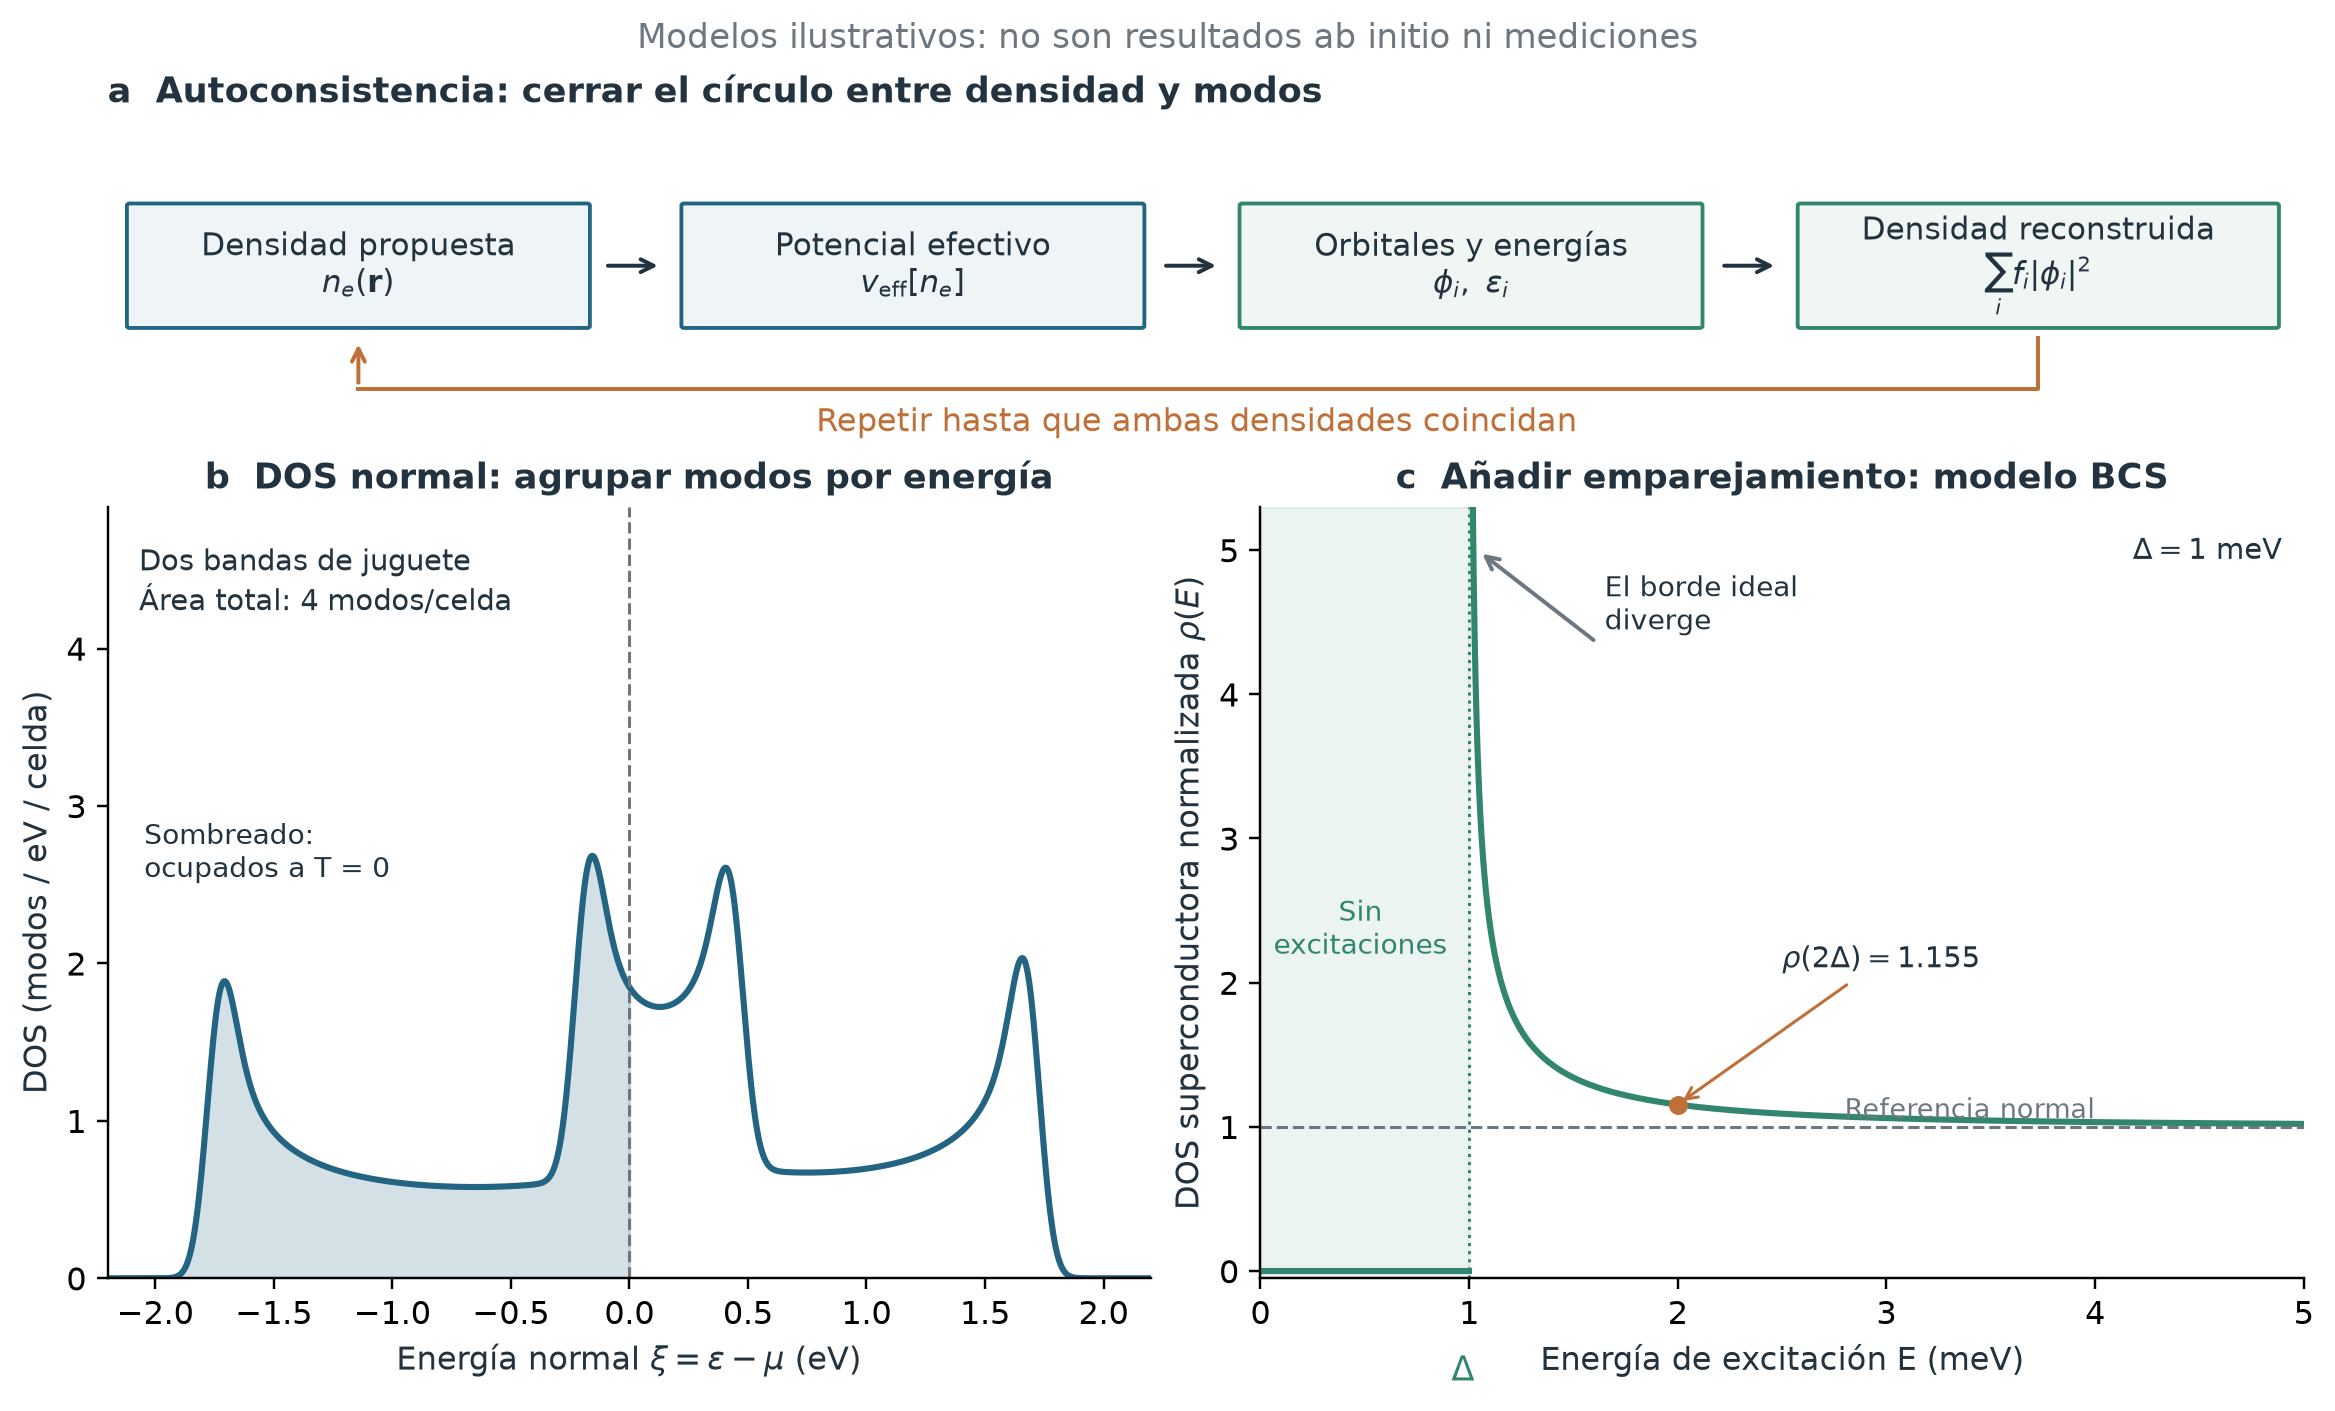
\includegraphics[width=1\linewidth,height=\textheight,keepaspectratio,alt={Figura E09.1. Arriba: la densidad y el potencial efectivo deben ser compatibles entre sí. Abajo: dos gráficos construidos para distinguir una DOS de modos electrónicos normales y una DOS superconductora normalizada. La primera usa dos bandas de juguete, con cuatro modos por celda incluyendo espín; la segunda usa BCS ideal con \textbackslash Delta=1 meV y DOS normal localmente constante. Son modelos ilustrativos, sin datos experimentales ni resultados ab initio. El borde BCS diverge y excede la escala vertical.}]{../figuras/E09_dft_dos.png}
\caption{Figura E09.1. Arriba: la densidad y el potencial efectivo deben
ser compatibles entre sí. Abajo: dos gráficos construidos para
distinguir una DOS de modos electrónicos normales y una DOS
superconductora normalizada. La primera usa dos bandas de juguete, con
cuatro modos por celda incluyendo espín; la segunda usa BCS ideal con
\(\Delta=1\) meV y DOS normal localmente constante. Son modelos
ilustrativos, sin datos experimentales ni resultados ab initio. El borde
BCS diverge y excede la escala vertical.}
\end{figure}

Un ejemplo discreto aclara el propósito. Repartamos un electrón entre
dos regiones y llamemos \(p\) y \(1-p\) a sus números medios. Definimos
una energía pedagógica, en eV,

\[
E(p)=p^2+(1-p)^2+(1-p)=2p^2-3p+2,
\qquad 0\le p\le1.
\tag{E09.a}
\]

El último término encarece ocupar la segunda región; los cuadrados
encarecen concentrar todo en una sola. Como \(E'(p)=4p-3\), el mínimo
está en \(p=3/4\), y \(E''(p)=4>0\). Se obtiene \(E(1/2)=1\),
\(E(3/4)=0.875\) y \(E(1)=1\) eV. El mínimo redistribuye el mismo
electrón: no cambia su carga ni crea partículas fraccionarias. Los
números \(3/4\) y \(1/4\) son promedios espaciales. Este funcional
inventado permite practicar la minimización; no es un cálculo DFT de un
material.

\subsection{E.7.2. Qué significa «funcional» en este
cálculo}\label{e.7.2.-quuxe9-significa-funcional-en-este-cuxe1lculo}

Con los núcleos fijos, una escritura útil de la energía electrónica es

\[
\mathcal E[n_e]=\mathcal F_{\rm el}[n_e]
+\int v_{\rm ion}(\mathbf r)n_e(\mathbf r)d^3r.
\tag{E09.b}
\]

\(v_{\rm ion}\) es la energía potencial de un electrón debida a los
iones. \(\mathcal F_{\rm el}\) reúne energía cinética e interacción
entre electrones; la energía entre núcleos puede sumarse y es constante
mientras sus posiciones estén fijas. Los corchetes indican que la
entrada es \textbf{el perfil completo} \(n_e\), no el valor de la
densidad en un solo punto.

Variar la densidad consiste en ensayar \(n_e+\epsilon\eta\), donde
\(\eta(\mathbf r)\) especifica dónde añadir y dónde retirar densidad, y
\(\epsilon\) fija la magnitud del cambio. Conservar los electrones exige
\(\int\eta\,d^3r=0\). Para variaciones admisibles alrededor de una
solución regular, la primera variación se anula bajo esa restricción.
Introduciendo un multiplicador \(\mu\) para el número de electrones se
escribe

\[
\delta\left(\mathcal E[n_e]-\mu\int n_e\,d^3r\right)=0,
\qquad \frac{\delta\mathcal E}{\delta n_e(\mathbf r)}=\mu.
\tag{E09.c}
\]

La derivada funcional indica el costo marginal de trasladar densidad
hacia una región. En el mínimo, una redistribución permitida no reduce
la energía a primer orden. En el ejemplo de dos regiones esto fue
exactamente imponer \(E'(p)=0\) conservando \(p+(1-p)=1\).

\subsection{E.7.3. Modos auxiliares, ocupaciones y
autoconsistencia}\label{e.7.3.-modos-auxiliares-ocupaciones-y-autoconsistencia}

Kohn y Sham construyen un sistema auxiliar de electrones sin interacción
explícita entre sí, sometidos a un potencial efectivo
\(v_{\rm eff}[n_e]\). Sus orbitales \(\phi_i\) permiten reconstruir la
densidad del sistema interactuante:

\[
\left[-\frac{\hbar^2}{2m_e}\nabla^2+v_{\rm eff}[n_e](\mathbf r)\right]\phi_i(\mathbf r)
=\varepsilon_i\phi_i(\mathbf r),
\qquad n_e(\mathbf r)=\sum_i f_i|\phi_i(\mathbf r)|^2.
\tag{E09.d}
\]

Aquí \(i\) incluye el espín; cada orbital está normalizado y
\(0\le f_i\le1\) es su ocupación media. Si se agrupan dos espines en un
único orbital espacial, aparece un factor dos. \(v_{\rm eff}\) incluye
el potencial iónico, la interacción electrostática media y una
contribución de intercambio y correlación, que se aproxima en cálculos
habituales. La \textbf{autoconsistencia} cierra el círculo: proponer
densidad, construir potencial, calcular orbitales, reconstruir densidad
y repetir hasta que ambas coincidan dentro de la precisión elegida.
\href{https://hj.hi.is/masterscourse/KohnSham65.pdf}{Kohn y Sham, 1965}.

En un cristal periódico, el índice \(i\) se organiza en banda, vector de
onda y espín. El orbital es un modo electrónico disponible; \(f_i\) dice
cuánto se ocupa. Al agrupar sus energías se obtiene la DOS de
Kohn--Sham,

\[
D_{\rm KS}(\varepsilon)=\sum_i\delta(\varepsilon-\varepsilon_i),
\qquad N_e=\int D_{\rm KS}(\varepsilon)f(\varepsilon)d\varepsilon,
\tag{E09.e}
\]

cuando la ocupación depende sólo de la energía. Para un sistema finito,
\(D_{\rm KS}\) tiene unidades de modos por energía. Si se divide por el
número de celdas, la integral ocupada da electrones \textbf{por celda}.
\(n_e(\mathbf r)\) agrupa electrones por posición; \(D_{\rm KS}\) agrupa
modos por energía; \(f\) selecciona sus ocupaciones. Ninguna de las tres
cantidades sustituye a las otras.

\subsection{E.7.4. De la DOS normal a las excitaciones
superconductoras}\label{e.7.4.-de-la-dos-normal-a-las-excitaciones-superconductoras}

Los valores propios auxiliares son útiles para construir la estructura
de bandas y una aproximación de partida al espectro electrónico. No
constituyen, en general, todas las energías exactas de añadir o retirar
electrones del sistema interactuante. Además, un cálculo DFT normal no
incorpora por sí solo el emparejamiento superconductor.

Para mostrar qué información adicional hace falta, tomemos una DOS
normal aproximadamente constante cerca de \(\mu\) y añadamos un modelo
de emparejamiento BCS uniforme e isotrópico, sin corriente. Si \(\xi\)
es una energía electrónica relativa a \(\mu\), una excitación tiene
energía \(E=\sqrt{\xi^2+\Delta^2}\). El cambio de variable da
\(|d\xi/dE|=E/\sqrt{E^2-\Delta^2}\). Con la normalización espectral
habitual, la DOS superconductora relativa a la normal resulta

\[
\rho(E)=\begin{cases}
0,&0\le E<\Delta,\\
\displaystyle\frac{E}{\sqrt{E^2-\Delta^2}},&E>\Delta.
\end{cases}
\tag{E09.f}
\]

\(\Delta\) es aquí positivo. A \(E=2\Delta\),
\(\rho=2/\sqrt3\simeq1.155\); por debajo de \(\Delta\) no hay
excitaciones en este modelo ideal. El aumento junto al borde proviene de
reorganizar el espectro. \(\rho\) es adimensional: para obtener una
densidad absoluta de cuasipartículas hace falta la DOS normal de
referencia y declarar el conteo de espines y ramas. Tampoco indica
cuántas excitaciones se han creado: eso requiere su ocupación
\(f(E,t)\). La figura usa exclusivamente este límite BCS. El cálculo del
detector de \href{https://arxiv.org/html/2501.13791v3}{Simon et al.,
apéndice VII.3 de la versión arXiv v3} obtiene la DOS bajo corriente
mediante otra ecuación espectral.

DFT aporta una base material: densidad de equilibrio, energía, orbitales
y bandas. Para conocer vibraciones se necesita además la respuesta a
desplazamientos; para seguir el evento de detección se necesitan
ocupaciones que evolucionan, interacciones y variables del dispositivo.
Cada paso añade una pregunta física concreta.

\subsection{E.7.5. Actividad}\label{e.7.5.-actividad}

\Needspace{4\baselineskip}

\textbf{E09.A1, 4 puntos.} En el ejemplo discreto, reemplazar el costo
de la segunda región por \(0.4(1-p)\) eV. Hallar el mínimo en
\(0\le p\le1\), comprobar la curvatura y expresar los números medios de
electrones en ambas regiones.

\textbf{Respuesta E09.A1:} \emph{Escribir aquí.}

\Needspace{4\baselineskip}

\textbf{E09.A2, 3 puntos.} Un gráfico tiene ejes energía y
modos/(eV·celda). Otro tiene posición y electrones/nm\(^3\). Identificar
cuál puede ser \(D_{\rm KS}\) y cuál \(n_e\), y explicar qué dato falta
para contar electrones ocupados a partir del primero.

\textbf{Respuesta E09.A2:} \emph{Escribir aquí.}

\Needspace{4\baselineskip}

\textbf{E09.A3, 3 puntos.} Corregir: «una DOS normal calculada por DFT
ya proporciona el gap superconductor y el número de cuasipartículas
después de absorber un fotón».

\textbf{Respuesta E09.A3:} \emph{Escribir aquí.}

\textbf{Condición esencial:} separar densidad espacial, modos
disponibles y ocupaciones, e identificar la información adicional del
modelo superconductor. Los cálculos pequeños y ambas curvas de la figura
se construyen aquí para enseñar estas diferencias.

\Needspace{14\baselineskip}

\bigskip

\section{E.8. DFPT: de mover un átomo a transferir energía ---
E10}\label{e.8.-dfpt-de-mover-un-uxe1tomo-a-transferir-energuxeda-e10}

\textbf{Revisión: r1. Estado: ABIERTO. Meta:} distinguir rigidez, conteo
de vibraciones y peso electrón--fonón, y leer cómo entran en una tasa.

\subsection{E.8.1. Introducción: quién determina los
resortes}\label{e.8.1.-introducciuxf3n-quiuxe9n-determina-los-resortes}

Una vibración de un sólido desplaza sus átomos. Ese desplazamiento
modifica el potencial que sienten los electrones; la densidad
electrónica responde y cambian las fuerzas sobre los átomos.
\textbf{DFPT}, teoría de perturbaciones del funcional de la densidad,
calcula esa respuesta alrededor de un equilibrio DFT. El nombre
«perturbación» indica que se estudia el efecto de un cambio pequeño, no
que el material deba estar desordenado.

Para una coordenada atómica \(u\), la respuesta lineal de la densidad es
\(n_e(\mathbf r;u)=n_e(\mathbf r;0)+u\,\partial_u n_e(\mathbf r;0)+\cdots\).
La posición \(\mathbf r\) recorre el espacio; \(u\) parametriza cuánto
se desplazó el átomo. La derivada \(\partial_u n_e\) es un perfil
espacial de respuesta. Se calcula incluyendo el cambio inducido del
potencial: desplazar los iones dejando la densidad congelada daría otra
rigidez.

Si \(\mathcal U(u)\) es la energía total con los electrones equilibrados
para cada \(u\), cerca de una geometría sin fuerza neta,

\[
\mathcal U(u)=\mathcal U_0+\frac12Ku^2+\cdots,
\qquad F_u=-\frac{d\mathcal U}{du}\simeq-Ku,
\qquad \omega^2=\frac{K}{M}.
\tag{E10.a}
\]

Se recupera un resorte, pero ahora su constante proviene de la energía
electrónica e iónica. Para muchas coordenadas, \(K\) se convierte en la
matriz de segundas derivadas; dividir cada entrada por
\(\sqrt{M_I M_J}\) produce la matriz dinámica, cuyos autovalores son
\(\omega^2\). Los autovectores indican qué átomos se mueven y en qué
dirección. Ésta es la conexión entre respuesta electrónica y modos
normales. \href{https://arxiv.org/pdf/cond-mat/0012092}{Baroni et al.,
secciones II.A y II.C}.

\begin{figure}
\centering
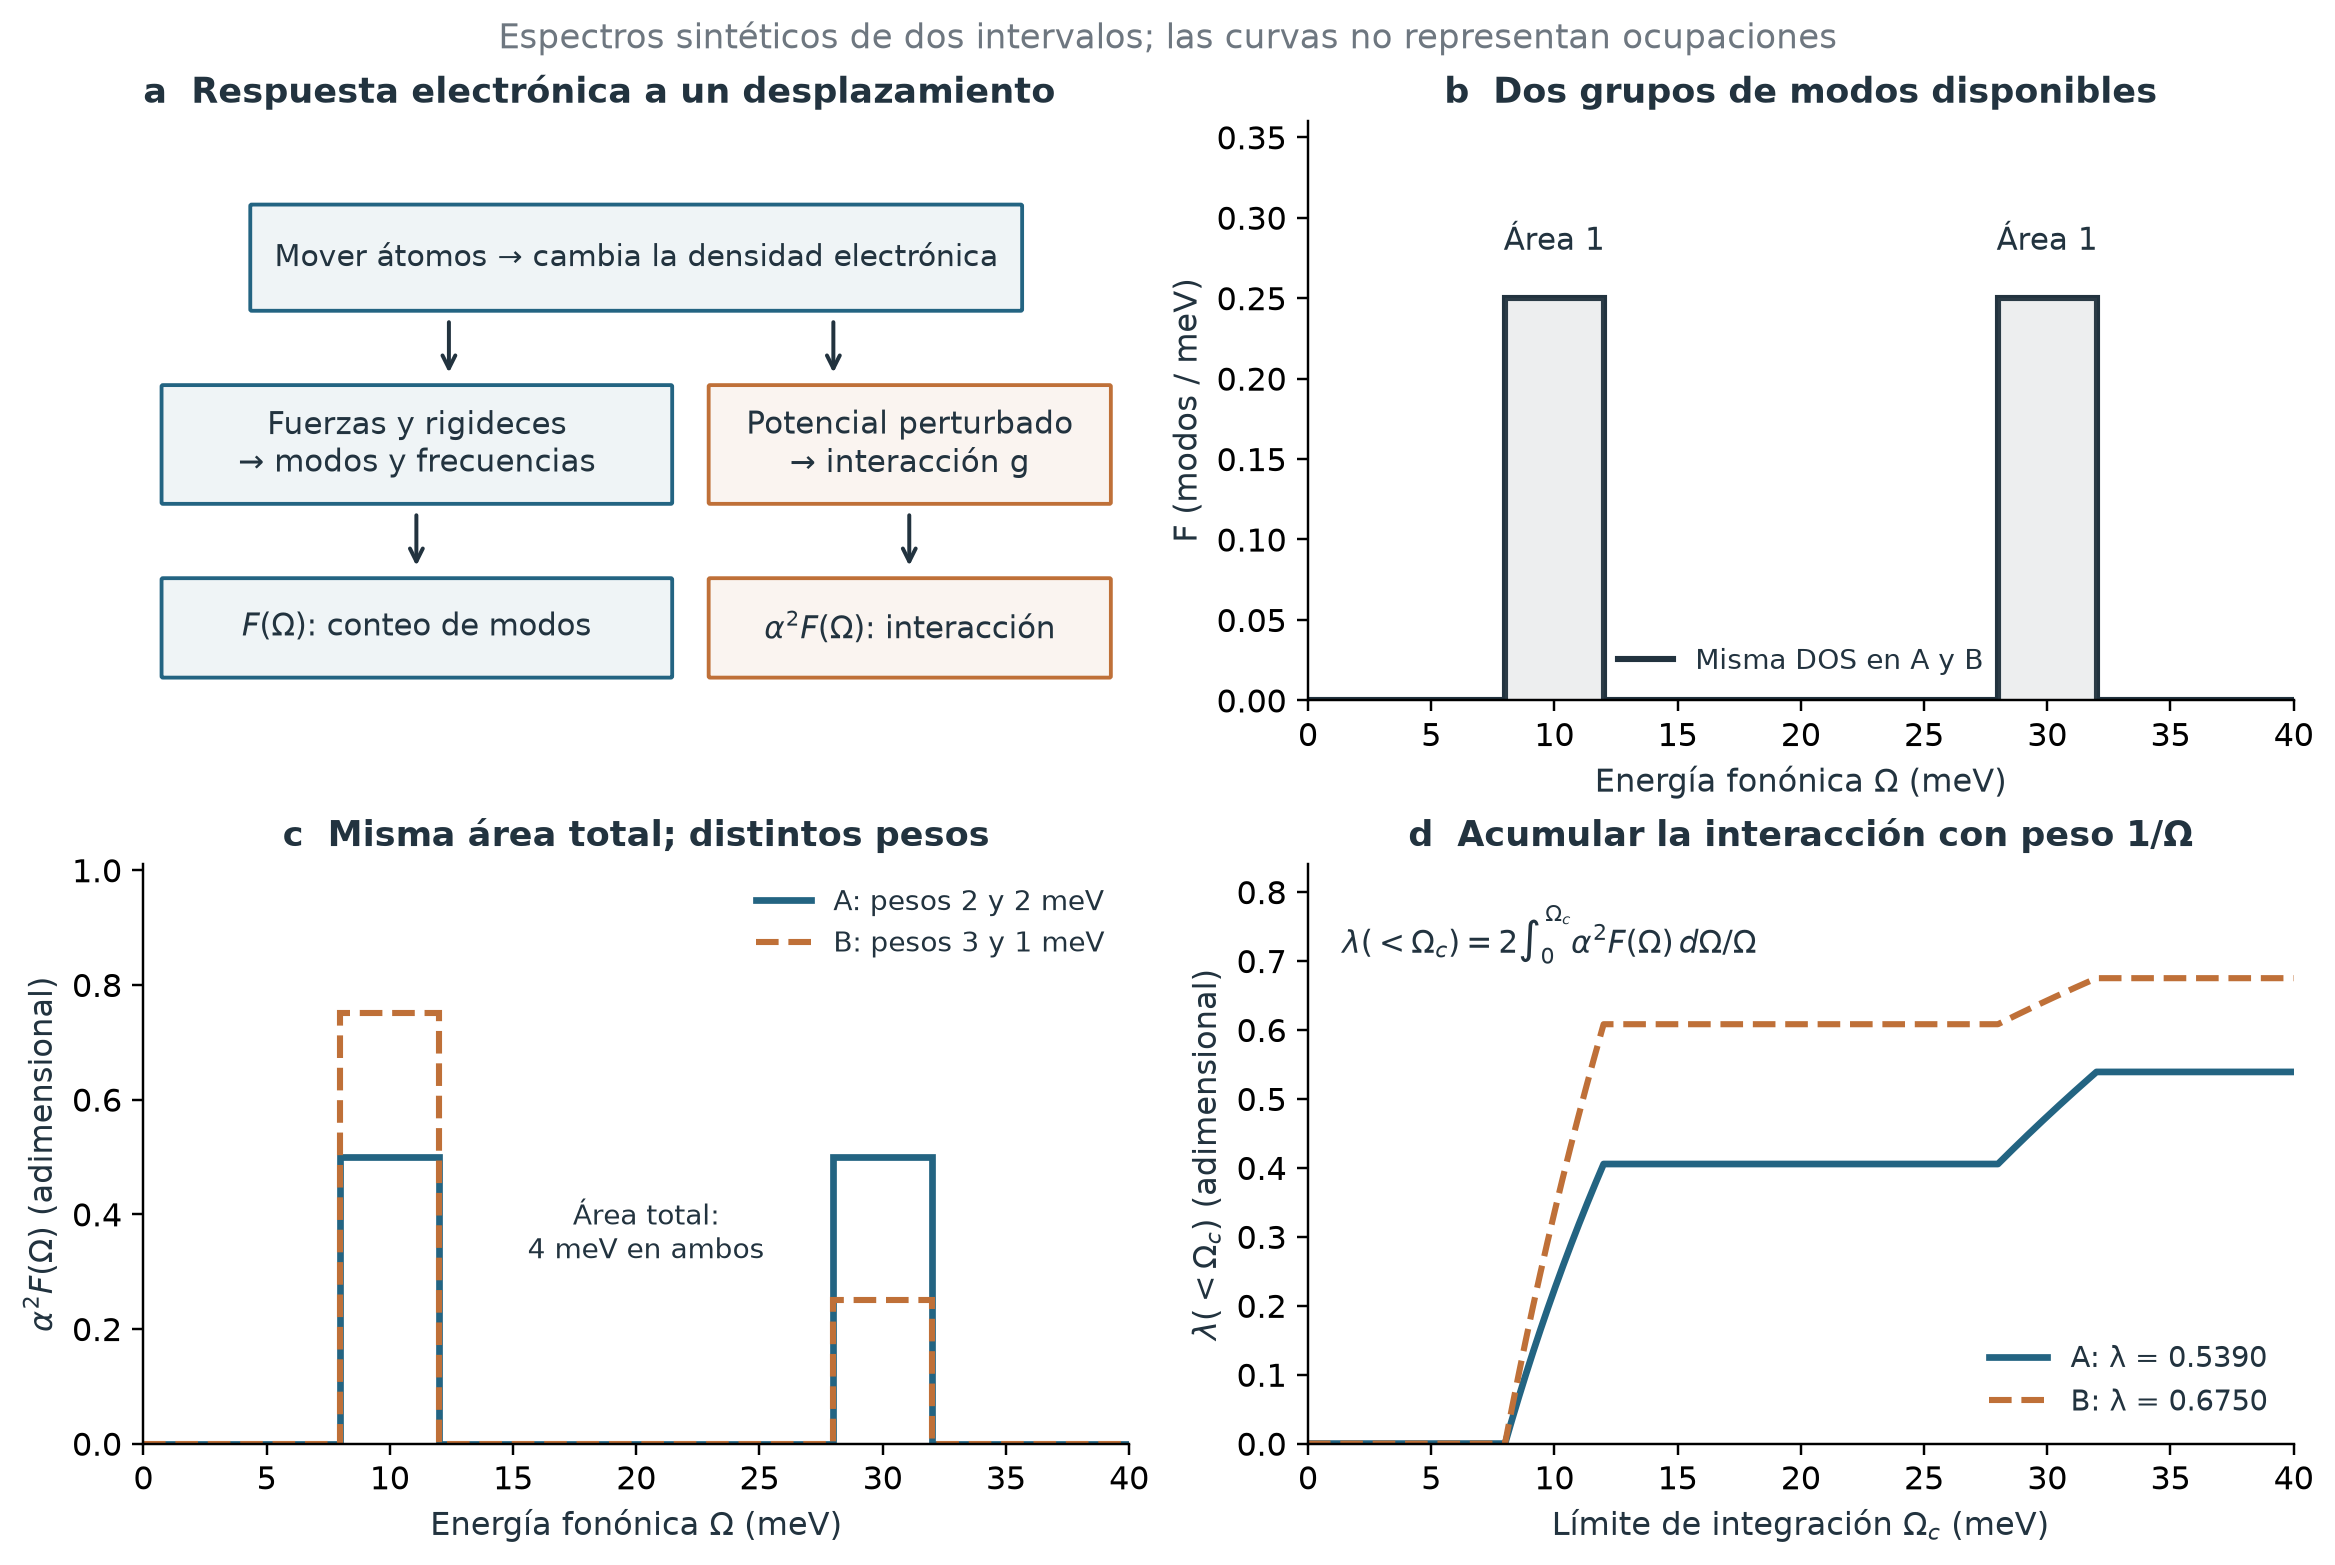
\includegraphics[width=1\linewidth,height=\textheight,keepaspectratio,alt={Figura E10.1. Ejemplo espectral construido, sin datos de un material: dos grupos de modos ocupan los intervalos 8--12 y 28--32 meV. Los casos A y B tienen exactamente la misma DOS y la misma área total de \textbackslash alpha\^{}2F, pero distribuyen de distinta manera sus pesos de interacción. El acumulado \textbackslash lambda(\textless\textbackslash Omega) permite ver cuánto aporta cada intervalo al acoplamiento total. Ninguna altura representa una ocupación fonónica.}]{../figuras/E10_dfpt_a2f.png}
\caption{Figura E10.1. Ejemplo espectral construido, sin datos de un
material: dos grupos de modos ocupan los intervalos 8--12 y 28--32 meV.
Los casos A y B tienen exactamente la misma DOS y la misma área total de
\(\alpha^2F\), pero distribuyen de distinta manera sus pesos de
interacción. El acumulado \(\lambda(<\Omega)\) permite ver cuánto aporta
cada intervalo al acoplamiento total. Ninguna altura representa una
ocupación fonónica.}
\end{figure}

\subsection{E.8.2. Una vibración puede acoplar mucho o
poco}\label{e.8.2.-una-vibraciuxf3n-puede-acoplar-mucho-o-poco}

La frecuencia de un modo no determina por sí sola cuánto afecta a los
electrones. Sea \(Q_\nu\) una coordenada normal con unidades de longitud
y masa efectiva \(M_\nu\). La escala cuántica de su desplazamiento es
\(Q_{\rm zp}=\sqrt{\hbar/(2M_\nu\omega_\nu)}\). La perturbación del
potencial conecta un modo electrónico inicial \(i\) con otro final \(j\)
mediante

\[
g_{ji,\nu}=Q_{\rm zp}
\left\langle\phi_j\left|\frac{\partial v_{\rm eff}}{\partial Q_\nu}\right|\phi_i\right\rangle.
\tag{E10.b}
\]

El corchete es un elemento de matriz: pondera espacialmente la
perturbación con los dos orbitales. Su unidad es energía/longitud;
multiplicarlo por \(Q_{\rm zp}\) da una energía. Las probabilidades de
transición contienen \(|g|^2\). En un cristal, los índices incluyen
bandas y vectores de onda. Esta escritura con masa efectiva es una
reducción a una coordenada normal; la documentación de
\href{https://www.quantum-espresso.org/Doc/ph_user_guide/node19.html}{Quantum
ESPRESSO, ecuación (1)} precisa su convención para masas y
polarizaciones.

La DOS fonónica \(F(\Omega)\) cuenta modos por intervalo de energía, con
\(\Omega=\hbar\omega\). La función de Eliashberg \(\alpha^2F(\Omega)\)
reúne esos intervalos ponderados por la interacción electrón--fonón y la
disponibilidad de estados electrónicos cerca del nivel de Fermi. Por eso
conocer sólo \(F\) no permite reconstruir \(\alpha^2F\). En la
convención energética usada aquí, \(\alpha^2F\) es adimensional y

\[
\lambda(<\Omega_c)=2\int_0^{\Omega_c}
\frac{\alpha^2F(\Omega)}{\Omega}\,d\Omega,
\qquad \lambda=\lambda(<\infty).
\tag{E10.c}
\]

\(\lambda\) es adimensional. La expresión coincide con la definición
posterior a la ecuación (2) de
\href{https://arxiv.org/html/2501.13791v3}{Simon et al., versión arXiv
v3}, y con
\href{https://www.quantum-espresso.org/Doc/ph_user_guide/node19.html}{Quantum
ESPRESSO, ecuación (5)} usando consistentemente el eje energético. Una
tabla externa necesita sus propias unidades y normalización declaradas.

\subsection{E.8.3. Ejemplo resuelto: misma DOS, distinta
interacción}\label{e.8.3.-ejemplo-resuelto-misma-dos-distinta-interacciuxf3n}

Construyamos dos perfiles \(p_1\) y \(p_2\), cada uno con área uno.
\(p_1=1/(4\,\mathrm{meV})\) entre 8 y 12 meV y cero fuera; \(p_2\) vale
lo mismo entre 28 y 32 meV. En el ejemplo \(F=p_1+p_2\) integra a
\textbf{dos modos representativos}: no es una DOS por átomo ni un conteo
completo de un cristal.

Definimos \(\alpha^2F=W_1p_1+W_2p_2\). Los pesos \(W_j\) tienen unidades
de energía. Para el caso A usamos \((W_1,W_2)=(2,2)\) meV y para B
\((3,1)\) meV. Ambos espectros tienen área \(W_1+W_2=4\) meV. Integrar
\(1/\Omega\) da un logaritmo; así,

\[
\begin{aligned}
\lambda_A&=2\left[\frac24\ln\frac{12}{8}
+\frac24\ln\frac{32}{28}\right]\simeq0.5390,\\
\lambda_B&=2\left[\frac34\ln\frac{12}{8}
+\frac14\ln\frac{32}{28}\right]\simeq0.6750.
\end{aligned}
\tag{E10.d}
\]

Todos los cocientes de energías son adimensionales. Tras el primer
intervalo, el acumulado vale 0.4055 en A y 0.6082 en B; el segundo
completa los valores anteriores. Transferir peso hacia energías bajas
aumenta esta integral porque contiene \(1/\Omega\). La diferencia no
proviene de haber añadido modos o fonones. Tampoco basta \(\lambda\)
para determinar una temperatura crítica: se necesitaría, entre otra
información, la distribución completa de energías de interacción y un
tratamiento de la repulsión electrónica.

En el límite de líneas estrechas, \(p_j\to\delta(\Omega-\Omega_j)\) y se
recupera \(\lambda=2\sum_j W_j/\Omega_j\). La figura conserva anchos
finitos; sus números corresponden a los logaritmos de E10.d, no a
sustituir sin más cada intervalo por su centro.

\subsection{E.8.4. Qué permite calcular en un
detector}\label{e.8.4.-quuxe9-permite-calcular-en-un-detector}

Una cuasipartícula de energía \(E\) puede emitir un fonón de energía
\(\Omega\) y pasar a \(E-\Omega\). En el modelo BCS con gap
\(\Delta>0\), el destino exige \(E-\Omega\ge\Delta\). Llamamos
\(f(E,t)\) a la ocupación media de un modo de cuasipartícula con energía
\(E\), con \(0\le f\le1\); no cuenta excitaciones por intervalo.
\(\Gamma_{\rm em}(E)\) será su tasa de salida por emisión. Omitimos el
argumento temporal al escribir los factores a un mismo instante. Con
ocupaciones fonónicas despreciables y cuasipartículas diluidas, la
contribución de pérdida por emisión de la ecuación (1a) de Simon et al.,
usando su núcleo (6b), se reduce a

\[
\left.\frac{\partial f(E)}{\partial t}\right|_{\rm pérdida,em}
\simeq-\Gamma_{\rm em}(E)f(E),
\tag{E10.e}
\]

\[
\Gamma_{\rm em}(E)=\frac{2\pi}{\hbar}
\int_0^{E-\Delta}d\Omega\,
\alpha^2F(\Omega)\rho(E-\Omega)
\left[1-\frac{\Delta^2}{E(E-\Omega)}\right].
\tag{E10.f}
\]

\(\rho\) es la DOS superconductora normalizada y el último factor
proviene de la composición electrónica y de hueco de las excitaciones.
La integral tiene unidades de energía; dividir por \(\hbar\) da una
tasa. Esta contribución no es la ecuación cinética completa: el mismo
nivel recibe partículas desde niveles superiores. A ocupaciones finitas
se restituyen los factores de bloqueo fermiónico, emisión estimulada y
absorción. La formulación citada supone isotropía y cuasipartículas bien
definidas, y sus ecuaciones locales omiten difusión.
\href{https://arxiv.org/html/2501.13791v3}{Simon et al., ecuaciones (1a)
y (6b), arXiv v3}.

Un cálculo de umbral permite leer la figura sin resolver la dinámica.
Elijamos \(\Delta=1\) meV y \(E=16\) meV: sólo se pueden emitir fonones
con \(\Omega\le15\) meV. Se abre todo el primer intervalo del ejemplo y
ninguno del segundo. En ese intervalo, \(\alpha^2F_B/\alpha^2F_A=3/2\).
Si ambos casos tienen la misma \(\Delta\) y la misma \(\rho\), la tasa
de pérdida calculada con E10.f es exactamente 1.5 veces mayor en B. A
\(E=40\) meV ya contribuyen ambos intervalos y no se puede usar ese
único cociente. Este ejemplo muestra por qué una tasa depende del
espectro y de los destinos permitidos, no sólo de su área total ni de
\(\lambda\).

La ocupación fonónica \(n(\Omega,t)\) responde a otra pregunta: cuántos
cuantos hay por modo. Si \(g_{\rm ph}(\Omega)\) es la DOS \textbf{por
volumen y por energía}, la energía vibratoria de excitaciones por
volumen es

\[
u_{\rm ph}(t)=\int_0^\infty
g_{\rm ph}(\Omega)\,\Omega\,n(\Omega,t)d\Omega.
\tag{E10.g}
\]

El producto se lee «modos por volumen e intervalo» por «energía por
cuanto» por «cuantos por modo». La energía de punto cero se omite al
contar excitaciones. \(F\) organiza modos, \(\alpha^2F\) pesa su
interacción y \(n\) fija sus ocupaciones. DFPT proporciona los dos
primeros ingredientes materiales; las ecuaciones cinéticas añaden la
evolución tras el fotón. Para llegar a una señal eléctrica también hay
que describir condensado, transporte y circuito.

\subsection{E.8.5. Actividad}\label{e.8.5.-actividad}

\Needspace{4\baselineskip}

\textbf{E10.A1, 4 puntos.} Para líneas estrechas en \(\Omega_1=5\) meV y
\(\Omega_2=20\) meV, con \(W_1=1\) meV y \(W_2=2\) meV, calcular
\(\lambda\). Transferir después \(0.5\) meV de peso del segundo modo al
primero y repetir. Explicar el cambio sin atribuirlo a crear nuevos
modos.

\textbf{Respuesta E10.A1:} \emph{Escribir aquí.}

\Needspace{4\baselineskip}

\textbf{E10.A2, 3 puntos.} Con \(E=10\) meV y \(\Delta=2\) meV, decidir
cuáles de los dos modos de la actividad anterior pueden recibir energía
por emisión de una cuasipartícula. Justificar con la energía del estado
final.

\textbf{Respuesta E10.A2:} \emph{Escribir aquí.}

\Needspace{4\baselineskip}

\textbf{E10.A3, 3 puntos.} Corregir: «si dos muestras tienen la misma
DOS fonónica, necesariamente tienen la misma función de Eliashberg y la
misma energía fonónica almacenada».

\textbf{Respuesta E10.A3:} \emph{Escribir aquí.}

\textbf{Condición esencial:} separar conteo, interacción y ocupación, y
usar conservación de energía para decidir qué transiciones se permiten.

\textbf{Referencia del ejemplo de investigación:} A. Simon et al.,
\emph{Ab initio modeling of nonequilibrium dynamics in superconducting
detectors and qubits},
\href{https://journals.aps.org/prb/abstract/10.1103/3m2k-mzr6}{Physical
Review B 112, 174512 (2025)}. Los números de ecuación indicados en esta
clase se cotejaron en
\href{https://arxiv.org/html/2501.13791v3}{arXiv:2501.13791v3}; su
figura 2 contiene espectros materiales calculados. Las figuras y los
números de esta clase son construcciones pedagógicas independientes y no
reproducen esos resultados.

\Needspace{14\baselineskip}

\bigskip

\section{E.9. Respuestas y próxima
revisión}\label{e.9.-respuestas-y-pruxf3xima-revisiuxf3n}

Hay 24 respuestas pendientes, tres por cada una de las ocho clases
activas. No se requiere resolver actividades de E02 o E08. Las
respuestas se escriben bajo su identificador en el documento editable;
la pauta y las calificaciones siguen pendientes de una entrega.

\textbf{Comentarios de aprendizaje:} \emph{Indicar qué símbolo, concepto
o paso necesita una explicación adicional.}

La siguiente revisión conservará las respuestas y modificará sólo el
material que las observaciones justifiquen. El estado de aprendizaje y
la revisión del contenido se registran por separado: una clase revisada
no se considera automáticamente aprobada.

\end{document}
